\chapter{Efficient Conflict Detection of Change-based Models}
\label{ch:conflict_detection}
  
In Chapter \ref{ch:model_differencing}, this work have demonstrated that  change-based model persistence can be exploited to speed up model differencing. In this Chapter, this work extends the proposed approach in Chapter \ref{ch:model_differencing} also by leveraging change-based model persistence to improve the performance of conflict detection in model versioning. The proposed approach can substantially reduce conflict detection time (up to 90\% in some experiments) compared to existing state-based and change-based conflict detection approaches. 

\section{Introduction}
\label{sec:introduction_7}
State-based and change-based model conflict detection have been discussed briefly in Sections \ref{sec:emfcompare_conflict_detection} and \ref{sec:emfstore_conflict_detection}. The state-based approach, represented by EMF Compare \cite{emfcompare2018developer}, does come with drawbacks. First, it cannot detect conflicts as accurate as change-based approach can as their changes are derived -- not the real historical changes. Second, EMF Compare uses 3-way model comparison \cite{emfcompare2018developer} thus hypothetically its conflict detection should perform relatively slower than the change-based approach, since it has to perform state-based model differencing twice to derive changes events: changes events between left and original versions, and change events between right and original versions. 

Change-based model conflict detection \cite{koegel2010operation}, represented by EMF Store \cite{emfstore2019what}, also has drawbacks. EMF Store purely works on comparing change events and detects conflicts based on predefined rules; it does not consider the eventual states of two versions that are being compared. Thus, two change events that modifies a same feature are considered in conflict even though both change events produce the same eventual states. In terms of performance, as has been presented in Chapter \ref{ch:model_differencing}, the change-based approach is faster than its state-based counterparts in model differencing. Thus, it is expected that it can also performs better that the state-based approach in detecting conflicts.
 
In this chapter, this work proposes a change-based approach that detects conflicts between two versions of model, not only based on the recent change events of the two versions, but also considers the eventual states of the elements affected by the change events. Thus, the performance and accuracy of model conflict detection can be improved compared to existing state-based and change-based approaches represented by EMF Compare and EMF Store respectively.

The rest of this chapter is structured as follows. Sections \ref{sec:emfcompare_conflict_detection} and \ref{sec:emfstore_conflict_detection} discuss briefly the conflict detection of in EMF Compare and EMF Store respectively. Sections \ref{sec:emf_cbp_conflict_detection} and Section \ref{sec:accuracy_of_conflict_detection} discuss our proposed approach to detect conflicts and its accuracy compared to EMF Compare and EMF Store. Section \ref{sec:evaluation_discussion} reports on the results of evaluation experiments used to evaluate the proposed approach. Section \ref{sec:conclusions_7} concludes this chapter.

\section{State-based Conflict Detection (EMF Compare)}
\label{sec:emfcompare_conflict_detection}

In this study, we select EMF Compare \cite{emfcompare2018developer} as an example tool to explain conflict detection in state-based model persistence. We also use it as a benchmark in the comparative evaluation of this paper. It is selected due to its maturity and ongoing development activity -- 4,682 commits and 103 releases on GitHub \cite{github2019emfcompare}. Another implementation of state-based conflict detection is EMF DiffMerge \cite{eclipse2019emfdiffmerge}. However, its comparison approach is similar to EMF Compare \cite{eclipse2019emfdiffmerge}, and it is less mature compared to EMF Compare -- only 442 commits and 20 releases on GitHub \cite{github2019emfdiffmerge}.

In state-based model comparison, a conflict occurs when the states of an element or a feature are different in two different versions of a model that are being compared. In other words, it can be said that the applied change events that cause the difference are in conflict since they produce two different states. State-based persistence does not record change events that cause the differences, thus the change events has to be identified through model differencing \cite{emfcompare2018developer,yohannis2019efficient}. 

Let's say that we have three versions of a model $M$, the original shared version $m_{o}$ and two other modified versions: the left version $m_{l}$ and the right version $m_{r}$. There are also two sets of identified change events, left change events $C_{L}$ and right change events $C_{R}$. These sets are obtained by differencing $m_{l}$ to $m_{o}$ and $m_{r}$ to $m_{o}$ using an LCS (Longest Common Subsequence) algorithm \cite{emfcompare2018developer,DBLP:journals/algorithmica/Meyers86}, where $C_{L}$ = $\{c_{l1}$, $c_{l2}$, ..., $c_{olm}\}$, $C_{R}$ = $\{c_{r1}$, $c_{r2}$, ..., $c_{rn}\}$, $m$ is number of left change events in $C_{L}$ or $m = |C_{L}|$, and $n$ is number of change events in $C_{R}$ or $n = |C_{R}|$. Applying $C_{L}$ to model $m_{o}$ transforms it into model $m_{l}$, and applying $C_{R}$ to model $m_{o}$ transforms it into model $m_{r}$. These derived change events are be used to detect conflicts using Equations (\ref{eq:state_real_conflict}), (\ref{eq:state_pseudo_conflict}), and (\ref{eq:state_nonapplicability_conflict}).  

If state-based model differencing is used to derive left change events $C_{L}$ from the left and original versions (Bob's and Jane's versions) in Figure \ref{fig:class_diagram_rpg}, the following change events are obtained. 
\begin{lstlisting}[firstnumber=1,style=eol,caption={The derived, minimal change events to produce the left version (Bob's version) in Figure \ref{fig:class_diagram_left} from the original version (Jane's version).},label=lst:cbp_left_state]
move target in attack.parameters from 1 to 2
set character.name from "Character" to "Hero"
set troll.name from "Troll" to "Ogre"
create leftGen type Generalization composite l1
set leftGen.general from null to character composite l1
set knight.generalization from null to leftGen composite l1
unset cast.name from "cast" to null composite l2
remove cast from giant.operations at 0 composite l2
delete cast composite l2
unset giant.name from "Giant" to null composite l3
remove giant from resource at 2 composite l3
delete giant composite l3
\end{lstlisting}

And following list is the derived change events for $C_{R}$ that are obtained from the right and original versions (Alice's and Jane's versions) in Figure \ref{fig:class_diagram_rpg}. 
\begin{lstlisting}[firstnumber=1,style=eol,caption={The derived, minimal change events to produce the right version (Alice's version) in Figure \ref{fig:class_diagram_right} from the original version (Jane's version).},label=lst:cbp_right_state]
move gem in attack.parameters from 0 to 1
set character.name from "Character" to "Hero"
set troll.name from "Troll" to "Orc"
remove smash from knight.operations at 0 composite r1
add smash to giant.operations at 0 composite r1
create rightGen type Generalization composite r2
set rightGen.general to character composite r2
set mage.generalization to rightGen composite r2
remove cast from giant.operations at composite r3
add cast to mage.operations at 0 composite r3
\end{lstlisting}

Both Listings \ref{lst:cbp_left_state} and \ref{lst:cbp_right_state} are derived change events. They are minimal sequence of change events that can produce $m_{l}$ and $m_{r}$ from $m_{o}$ respectively, but not necessarily the real changes made by Bob and Alice. For example, Bob and Alice may have created and then deleted a new class in the process or modified a feature but later decided to set it back to its initial value.

\textbf{Real Conflict}. In state-based model comparison, two change events, $c_{l}$ and $c_{r}$, are in conflict if both are applied to a same element $e_{o}$ but produce two different eventual states where $!$ is used as the operator for expressing that two change events are in conflict (\ref{eq:state_real_conflict}). EMF Compare \cite{emfcompare2018developer} classifies this conflict as a \textsf{REAL} conflict. For example, Bob changed the \textsf{name} of \textsf{troll} to ``Ogre'' (Listing \ref{lst:cbp_left_state}) while Alice modified it to ``Orc'' (Listing \ref{lst:cbp_right_state}). 
\begin{equation} \label{eq:state_real_conflict}
e_{o} + c_{l} \not\equiv e_{o} + c_{r} \Rightarrow c_{l}\;!\;c_{r}
\end{equation} 
\textbf{Non-applicability}. A \textsf{REAL} conflict also occurs when applying a change event $c_{l}$ to element $e_{o}$ makes $c_{r}$ inapplicable to element $e_{o}$. Therefore, change events $c_{l}$ and $c_{r}$ are in conflict (\ref{eq:state_nonapplicability_conflict}). 
For instance, Alice moved operation \textsf{smash} from class \textsf{Knight} to class \textsf{Giant} (Listing \ref{lst:cbp_right_state}) but this class was deleted by Bob (Listing \ref{lst:cbp_left_state}). Deleting class \textsf{Giant} makes the move inapplicable. 
\begin{equation} \label{eq:state_nonapplicability_conflict}
(e_{o} + c_{r} \not\equiv e_{o}) \wedge (e_{o} + c_{l} + c_{r} \equiv e_{o} + c_{l}) \Rightarrow c_{l}\;!\;c_{r}
\end{equation}
\textbf{Pseudo Conflict}. A conflict is classified as \textsf{PSEUDO} if the eventual states produced are equivalent. The \textsf{PSEUDO} means the conflict can be automatically resolved by choosing any of the conflicting changes since any of the changes produces the same eventual states (\ref{eq:state_pseudo_conflict}) \cite{emfcompare2018developer}. Symbol $!_{p}$ is used as the operator for expressing that two change events are in \textsf{PSEUDO} conflict. For example, both Bob and Alice changed the \textsf{name} of element \textsf{character} from ``Character'' to ``Hero'' (Listings \ref{lst:cbp_left_state} and \ref{lst:cbp_right_state}). 
\begin{equation} \label{eq:state_pseudo_conflict}
e_{o} + c_{l} \equiv e_{o} + c_{r} \Rightarrow c_{l}\;!_{p}\;c_{r}
\end{equation} 


\begin{table*}[ht]
  \centering
  \caption{Conflicting change events identified using EMF Compare based on the case in Figure \ref{fig:class_diagram_rpg}.}
  \begin{scriptsize}
  \label{table:emfc_conflicts}
  \begin{tabular}{|p{0.04\linewidth}|p{0.37\linewidth}|p{0.37\linewidth}|
      p{0.11\linewidth}|}
    \hline
    \textbf{ID} & 
    \textbf{Left Change Events (Bob)} & 
    \textbf{Right Change Events (Alice)} & 
    \textbf{Type}\\ 
    \hline
    EC1 & 
    set character.name from "Character" to "Hero" & 
    set character.name from "Character" to "Hero" & 
    real \\
    \hline
    EC2 & set troll.name from "Troll" to "Ogre" & 
    set troll.name from "Troll" to "Orc & 
    real \\ 
    \hline
    EC3 & 
    delete cast
    & 
    \begin{minipage}[t]{\linewidth}
      \raggedright
      \begin{itemize}[leftmargin=0pt]
        \setlength
        \item[] remove cast from giant.operations at 0
        \item[] add cast to mage.operations at 0
      \end{itemize}
    \end{minipage}
    & 
    real, non-applicability\\
    \hline
    EC4 & 
    delete giant
    & 
    \begin{minipage}[t]{\linewidth}
      \raggedright
      \begin{itemize}[leftmargin=0pt]
        \setlength
        \item[] remove smash from knight.operations at 0
        \item[] add smash to giant.operations at 0
      \end{itemize}
    \end{minipage}
    & 
    real, non-applicability\\
    \hline
  \end{tabular}
\end{scriptsize}
\end{table*}

Using Equations (\ref{eq:state_real_conflict}), (\ref{eq:state_nonapplicability_conflict}), and (\ref{eq:state_pseudo_conflict}) and information in Listings \ref{lst:cbp_left_state} and \ref{lst:cbp_right_state}, four conflicts can be identified -- presented in Table \ref{table:emfc_conflicts} along with their conflicting change events. Conflict \textsf{EC1} is a \textsf{pseudo} conflict since both modify the same class \textsf{character}'s feature \textsf{name} resulting the same end states, ``Hero'' or ``Hero''. Conflict \textsf{EC2} is a \textsf{REAL} conflict. Applying changing \textsf{troll}'s \textsf{name} to ``Ogre'' and \textsf{troll}'s \textsf{name} to ``Orc'' produces two different states -- ``Ogre'' and ``Orc''. Conflicts \textsf{EC3} and \textsf{EC4} are \textsf{REAL} non-applicability conflicts since if operation \textsf{cast} is deleted first then it cannot be moved -- removed and added -- from class \textsf{giant}'s \textsf{operations} to class \textsf{mage}'s \textsf{operations}, and if class \textsf{giant} is deleted first then operation \textsf{smash} cannot be moved -- removed and added -- from  class \textsf{knight}'s \textsf{operations} to class \textsf{giant}'s \textsf{operations}.

Conflict detection in state-based comparison might not be accurate since the derived differences/change events might not reflect the real historical changes of a model. For example, EMF Compare \cite{emfcompare2018developer} does not detect that Alice and Bob modified the same element -- parameter \textsf{target} -- as indicated by line 29 in List. \ref{lst:cbp_right} and line 35 in List. \ref{lst:cbp_left}. Using an LCS algorithm, the derived change events related to the feature \textsf{parameters} of element \textsf{attack}, which if presented as change events, are expressed as [\textsf{\small \textbf{move} target \textbf{in} attack.parameters \textbf{from} 1 \textbf{to} 2}] for Bob's version and [\textsf{\small \textbf{move} gem \textbf{in} attack.parameters \textbf{from} 1 \textbf{to} 2}] for Alice's version. Using (\ref{eq:state_real_conflict}), both change events are not in conflict since both change events modify two different elements, \textsf{target} and \textsf{gem}. The result is different if change-based approach is employed to detect conflicts using the change event records in Listings \ref{lst:cbp_left} and \ref{lst:cbp_right} which is explained in Section \ref{sec:emfstore_conflict_detection}.

\section{Change-based Conflict Detection (EMF Store)}
\label{sec:emfstore_conflict_detection}
EMF Store \cite{koegel2010emfstore} is an open-source tool that implements change-based model persistence for EMF models. It is a collaborative repository and versioning system that is specifically designed for models to answer existing versioning systems, such as Git and SVN, that focus heavily on text-based files \cite{emfstore2019what}. EMF Store follows the following rules to identify conflict between change events \cite{koegel2010operation}. 

\textbf{Non-commutability}. In EMF Store, change events $c_{l}$ and $c_{r}$ are in conflict if applying them in different order to a same element $e_{o}$ produces two different eventual states \cite{koegel2010operation}. For example, Alice changed the \textsf{name} of class \textsf{Troll} to ``Orc'' (Listing \ref{lst:cbp_right}) while Bob renamed it to ``Ogre'' (Listing \ref{lst:cbp_left}). Applying Alice's change first to Bob's change results in the class' \textsf{name} equals to ``Ogre'', or ``Orc'' if the order is reversed.
\begin{equation} \label{eq:change_noncommutability}
e_{o} + c_{l} + c_{r} \not\equiv e_{o} + c_{l} + c_{r} \Rightarrow c_{l}\;!\;c_{r}
\end{equation}  
However, after examining the implementation \cite{eclipse2019emfstore}, even though two different change events produce equivalent eventual states, both change events are still treated in conflict by EMF Store (\ref{eq:ecbp_equal_end_states}). For example, both Bob and Alice changed the \textsf{name} of element \textsf{character} from ``Character'' to ``Hero'' (Listing \ref{lst:cbp_left} line \ref{line:cbp_left_34} and Listing \ref{lst:cbp_right} line \ref{line:cbp_right_39}). The reason is if we apply Bob's set event first, it changes \textsf{character}'s \textsf{name} from ``Character'' to ``Hero''. It is important to notice that after applying Bob's set event, the eventual value of \textsf{character}'s \textsf{name} is ``Hero''. Applying Alice's set event with previous value ``Character'' is inapplicable since it makes the sequence of the change events inconsistent; Bob's set event produces eventual value ``Hero'' which is not the previous value changed by Alice's set event, which is ``Character''. The same inconsistency still occurs even we apply these set events in different order.
\begin{equation} \label{eq:ecbp_equal_end_states}
\begin{split}
e_{o} + c_{l} + c_{r} \equiv e_{o} + c_{l} + c_{r} \Rightarrow c_{l}\;!\;c_{r}
\end{split}
\end{equation} 
Moreover, a conflict still occurs even though two different sets of change events, $C_{L}$ and $C_{R}$, produce eventual states that are equal to their initial states (\ref{eq:ecbp_equal_to_original_states}). For example, if both Bob and Alice alter \textsf{character}'s \textsf{name} from ``Character'' to ``Hero'' and then modify it back to ``Character'', both sets of change events are also treated in conflict.
\begin{equation} \label{eq:ecbp_equal_to_original_states}
\begin{split}
e_{o} + C_{L} + C_{R} \equiv e_{o} + C_{R} + C_{L} \equiv e_{o}  \Rightarrow C_{L}\;!\;C_{R}
\end{split}
\end{equation} 
\textbf{Co-modification}. Thus, this leads to a new definition that a conflict occurs when two different change events modify a same element or feature regardless of the eventual states that they produce. 
\begin{equation} \label{eq:change_comodifiabilty}
(e_{o} + c_{l} \equiv e_{o} + c_{r}) \vee (e_{o} + c_{l} \not\equiv e_{o} + c_{r}) \Rightarrow c_{l}\;!\;c_{r}
\end{equation} 
\textbf{Non-applicability}. This non-applicability rule is the same with the non-applicability rule in the state-based conflict detection. Essentially, a conflict occurs when applying a change event $c_{l}$ to element $e_{o}$ makes $c_{r}$ inapplicable to element $e_{o}$. For instance, Alice moved operation \textsf{smash} from class \textsf{Knight} to class \textsf{Giant} (Listing \ref{lst:cbp_right}) but this class was deleted by Bob (Listing \ref{lst:cbp_left}). Deleting class \textsf{Giant} makes the move inapplicable. 
\begin{equation} \label{eq:change_nonapplicability}
(e_{o} + c_{r} \not\equiv e_{o}) \wedge (e_{o} + c_{l} + c_{r} \equiv e_{o} + c_{l}) \Rightarrow c_{l}\;!\;_{r}
\end{equation}
\textbf{Composite}. If change event $c_{l}$ is in conflict with change event $c_{r}$ where $c_{r}$ is a member of a set of composite change event $cc_{r}$ then change event $c_{l}$ is also in conflict with each change event $c_{n}$ in composite change event $cc_{r}$. For example, the deletion of class \textsf{Giant} is part of composite event \textsf{l2} (Listing \ref{lst:cbp_left}) and the addition of operation \textsf{smash} to class \textsf{Giant} is part of composite event \textsf{r1} (Listing \ref{lst:cbp_right}). Since they are in conflict according to (\ref{eq:change_nonapplicability}), all other change events in their composite events, \textsf{l2} and \textsf{r1}, are also in conflict.
\begin{equation} \label{eq:change_composite}
c_{l}\;!\;c_{r} \wedge c_{r} \in cc_{r} \Rightarrow c_{l}\;!\; \forall c_{rn} | c_{rn} \in cc_{r}
\end{equation}

\begin{table*}[ht]
  \centering
  \caption{Conflicting change events identified using EMF Store in Listings \ref{lst:cbp_right} and \ref{lst:cbp_left}.}
  \label{table:conflicts_emfs}
\begin{scriptsize}
  \begin{tabular}{|p{0.04\linewidth}|p{0.37\linewidth}|p{0.37\linewidth}|
      p{0.11\linewidth}|}
    \hline
    \textbf{ID} & 
    \textbf{Left Change Events (Bob)} & 
    \textbf{Right Change Events (Alice)} & 
    \textbf{Type}\\ 
    \hline
    ES1 & 
    \begin{minipage}[t]{\linewidth}
      \raggedright
      \begin{itemize}[leftmargin=0pt]
        \setlength
        \item[] set troll.generalization from null to left
        Gen
        \item[] unset troll.generalization from leftGen
        to null
        \item[] set knight.generalization from null
        to leftGen
      \end{itemize}
    \end{minipage} & 
    \begin{minipage}[t]{\linewidth}
      \raggedright
      \begin{itemize}[leftmargin=0pt]
        \setlength
        \item[] set troll.generalization from null to
        rightGen
        \item[] unset troll.generalization from rightGen
        to null
        \item[] set mage.generalization from null to
        rightGen
      \end{itemize}
    \end{minipage} & 
    co-modification,
    composite \\
    \hline
    ES2 & set character.name from "Character"
    to"Hero" & 
    set character.name from "Character"
    to "Hero" & 
    co-modification \\ 
    \hline
    ES3 & 
    move target in attack.parameters from
    1 to 2
    & 
    move target in attack.parameters from
    1 to 0
    & 
    non-applicability\\
    \hline
    ES4 & 
    \begin{minipage}[t]{\linewidth}
      \raggedright
      \begin{itemize}[leftmargin=0pt]
        \setlength
        \item[] unset cast.name from "cast" to null
        \item[] remove cast from giant.operations at 0
        \item[] delete cast type Operation
        \item[] unset giant.name from "Giant" to null
        \item[] delete giant
      \end{itemize}
    \end{minipage}
    & 
    \begin{minipage}[t]{\linewidth}
      \raggedright
      \begin{itemize}[leftmargin=0pt]
        \setlength
        \item[] remove cast from giant.operations at 0
        \item[] add cast to mage.operations at 0
        \item[] remove smash from knight.operations at 0
        \item[] add smash to giant.operations at 1
      \end{itemize}
    \end{minipage}
    & 
    non-applicability, composite\\
    \hline
    ES5 & 
    set troll.name from "Troll" to "Ogre" & 
    set troll.name from "Troll" to "Orc" & 
    co-modification\\ 
    \hline
  \end{tabular}
\end{scriptsize}
\end{table*}

In change-based conflict detection, all change events applied to a model are readily available, thus the change events do not need to be derived trough a diffing process. The availability of real historical changes can improve the accuracy of change detection since elements that have been changed can be identified according to fact -- not derivation. In consequence, it can detect conflicts that cannot be detected by state-based conflict detection. For example, in Listing \ref{lst:cbp_right} line 31, parameter \textsf{target} has been moved from index 1 to 0, while in Listing \ref{lst:cbp_left} line 37, it was moved from index 1 to 2. Since both change events modified the same parameter \textsf{target}, both change events can be identified in conflict using (\ref{eq:change_comodifiabilty}); the same parameter \textsf{target} is modified by two different change events. 

The drawback of EMF Store is that it treats two change events that modify the same element as they are in conflict regardless of the end states that they produce to the element \cite{DBLP:conf/sfm/BroschKLSWW12}. In common sense, two changes should not be in conflict if they are applied to a same element or feature and produce same eventual states. Moreover, EMF Store it does not have a classification that separates conflicts into \textsf{REAL} or \textsf{PSEUDO} conflicts, such as in EMF Compare, to automate conflict resolution. 

%For example, two change events in Listing \ref{lst:cbp_right} at line \ref{line:cbp_right_39} and Listing \ref{lst:cbp_left} at line \ref{line:cbp_left_35}, that change the same feature \textsf{name} from ``Character'' to the same value ``Hero'', are treated in conflict (Table \ref{table:conflicts_emfs} id ES2) using (\ref{eq:change_comodifiabilty}). EMF Compare classifies this kind of conflict as \textsf{PSEUDO} conflict which can be automatically resolved in merging only by selecting one of the conflicting change events and ignoring the other one.

Excluding eventual states in detecting conflicts also causes all change events related to \textsf{troll}'s \textsf{generalization} to be in conflict; all the feature's left-side events are in conflict with all its right-side events (Table \ref{table:conflicts_emfs}, ES1). Using the co-modification  (\ref{eq:change_comodifiabilty}) rule, we can detect that the setting and unsetting of \textsf{troll}' \textsf{generalization} to \textsf{leftGen} and \textsf{null} (Listing \ref{lst:cbp_left} lines \ref{line:cbp_left_33}, \ref{line:cbp_left_35}) are in conflict with the setting and unsetting of \textsf{troll}' \textsf{generalization} to \textsf{rightGen} and \textsf{null} (Listing \ref{lst:cbp_right} lines \ref{line:cbp_right_38}, \ref{line:cbp_right_40}). Moreoever, using composite (\ref{eq:change_composite}) rule, we can also identify that the setting of \textsf{knight}' \textsf{generalization} to \textsf{leftGen} (Listing \ref{lst:cbp_left} line \ref{line:cbp_left_36}) and the setting of \textsf{mage}' \textsf{generalization} to \textsf{rightGen} (Listing \ref{lst:cbp_right} line \ref{line:cbp_right_41}) are also part of the conflict ES1 since both events are in the same composite move events, \textsf{l1} and \textsf{r3}, with the unsetting of \textsf{troll}' \textsf{generalization} to  \textsf{null} (Listing \ref{lst:cbp_left} line \ref{line:cbp_left_35}, Listing \ref{lst:cbp_right} line \ref{line:cbp_right_38}).

In state-based conflict detection, case ES1 is not a conflict since the values of class \textsf{troll}'s feature \textsf{generalization} in the Jane's, Bob's, and Alice's versions are indentical -- all are null. Thus, there are no different \textit{derived} change events that modify class \textsf{troll}'s feature \textsf{generalization} in parallel. 

Conflict ES4 is a non-applicability, composite conflict. Moving element \textsf{smash} from class \textsf{knight} to class \textsf{giant} and moving element \textsf{cast} from class \textsf{giant} to class \textsf{mage} require the deletion of class \textsf{giant} to be executed later in order to be applicable. Conflict ES5 is can be detected with the co-modification  (\ref{eq:change_comodifiabilty}) rule. The states of \textsf{troll}'s \text{name} have been simultaneously modified to ``Ogre'' or ``Orc''.

\begin{table*}[ht]
  \centering
  \caption{The advantages and drawbacks of EMF Compare and EMF Store in detecting conflicts.}
  \label{tab:accuracy_emfcompare_emfstore}
  \begin{scriptsize}
  \begin{tabular}{|p{0.1\linewidth}|p{0.4\linewidth}|p{0.4\linewidth}|}
    \hline
    \textbf{Dimension}
    & \textbf{State-based Conflict Detection (EMF Compare)}
    & \textbf{Change-based Conflict Detection (EMF Store)}\\
    \hline
    \multicolumn{1}{|c|}{Advantages}
    &
    \begin{minipage}[t]{\linewidth}
      \raggedright
      \begin{itemize}[leftmargin=9pt]
        \setlength\itemsep{2pt}
        \item[-] detect \textsf{PSEUDO} conflict which can be automatically resolved when merging
        \item[-] conflicts detected are optimal since changes are derived thus avoid oversensitive conflict detection
        \item[]
      \end{itemize}
    \end{minipage}
    &
    \begin{minipage}[t]{\linewidth}
      \raggedright
      \begin{itemize}[leftmargin=9pt]
        \setlength\itemsep{2pt}
        \item[-] more accurate in detecting conflicts since changes are real history
        \item[-] in large models with moderate changes, it should perform faster than the state-based approach -- no need to derive changes since they are already available 
        \item[]
      \end{itemize} 
    \end{minipage}
    \\ 
    \hline
    \multicolumn{1}{|c|}{Drawbacks}
    &
    \begin{minipage}[t]{\linewidth}
      \raggedright
      \begin{itemize}[leftmargin=9pt]
        \setlength\itemsep{2pt}
        \item[-] less accurate in detecting conflicts since changes are derived -- not real changes
        \item[-] in large models, its performance should be slower the change-based approach since it performs 3-way comparison which requires 2-times model differencing to derive changes
        \item[-] in small models, it should perform faster than change-based approach
        \item[]
      \end{itemize}
    \end{minipage}
    &
    \begin{minipage}[t]{\linewidth}
      \raggedright
      \begin{itemize}[leftmargin=9pt]
        \setlength\itemsep{2pt}
        \item[-] treat all conflicts as \textsf{REAL} conflicts which demand user intervention for resolution
        \item[-] can be oversensitive in detecting conflicts since eventual states are not considered
        \item[-] in small models with excessive changes, it should perform slower than the state-based approach due to processing lots of change records
        \item[]
      \end{itemize} 
    \end{minipage}
    \\
    \hline                         
  \end{tabular}
\end{scriptsize}
\end{table*}

\subsection{Summary}
\label{sec:summary}
The summary of the advantages and drawbacks between EMF Compare and EMF Store in detecting conflicts are presented in Table \ref{tab:accuracy_emfcompare_emfstore}. The state-based approach, represented by EMF Compare \cite{emfcompare2018developer}, does come with drawbacks. First, it cannot detect conflicts as accurate as change-based approach can as their changes are derived -- not the real historical changes. Second, EMF Compare uses 3-way model comparison \cite{emfcompare2018developer} thus hypothetically its conflict detection should perform relatively slower than the change-based approach, since it has to perform state-based model differencing twice to derive changes events: changes events between left and original versions, and change events between right and original versions. 

Change-based model conflict detection \cite{koegel2010operation}, represented by EMF Store \cite{emfstore2019what}, also has drawbacks. EMF Store purely works on comparing change events and detects conflicts based on predefined rules; it does not consider the eventual states of two versions that are being compared. Thus, two change events that modifies a same feature are considered in conflict even though both change events produce the same eventual states. This condition can lead EMF Store to oversensitive conflict detection. 

\section{EMF CBP Conflict Detection}
\label{sec:emf_cbp_conflict_detection}

The model conflict detection proposed in this study basically performs similar procedure to the phases of change-based model differencing discussed in Chapter \ref{sec:change_based_approach_for_comparing_models} but with some modification. First, the conflict detection still performs the event loading and element tree construction phases, but the diff computation phase is replaced with conflict computation phase. Second, during element tree construction, the conflict detection maps change events to the elements, features, and values that the change events modify. The change event mapping and conflict computation are discussed in the following Sections.

\subsection{Change Event Mapping}
\label{sec:change_event_mapping}
Using the information contained in the change-based model representations in Listings \ref{lst:cbp_left} and \ref{lst:cbp_right}, we can construct an element tree as depicted in Figure \ref{fig:right_element_tree_diagram} using the construction method presented in Section \ref{sec:tree_construction}. During the the construction, change events in Listings \ref{lst:cbp_left} and \ref{lst:cbp_right} are mapped to the affected elements, features, and values which act as the keys of the mapping. The relationships are stored in attributes \textsf{leftEvents} and \textsf{rightEvents} of class \textsf{Element} and \textsf{leftEvents}, \textsf{rightEvents}, \textsf{leftValueEvents}, and \textsf{rightValueEvents} of class \textsf{Feature} in Figure \ref{fig:approach_class_diagram}. This registration forms many-to-many relationships between the keys and change events. In detail, the keys are \textsf{element} for elements, or a combination of \textsf{element-feature} for single-valued features or \textsf{element-feature-value} for multivalued-features. With this mapping, we can trace all events that affects certain elements, features, and values. The mapping of the events in Listings \ref{lst:cbp_left} and \ref{lst:cbp_right} is in Table \ref{tab:keyeventsmap}. The application of this mapping is presented in Section \ref{sec:delete_conflict}.

\begin{table*}[ht]
\centering
\caption{The mapping of elements, features, and values in Figure \ref{fig:right_element_tree_diagram} to the events that affect them.}
\label{tab:keyeventsmap}
  \begin{scriptsize}
\begin{sffamily}
\begin{tabular}{|m{0.30\linewidth}|m{0.275\linewidth}|m{0.275\linewidth}|}
\hline
\textbf{Key} & \textbf{Left Events} & \textbf{Right Events} \\ \hline
character                          & cl32, cl34                                & cr37, cr39                                 \\ \hline
character.name                     & cl34                                      & cr39                                       \\ \hline
attack                             & cl37                                      & cr31                                       \\ \hline
attack.parameters.target           & cl37                                      & cr31                                       \\ \hline
target                             & cl37                                      & cr31                                       \\ \hline
trcll                              & cl33, cl35                                & cr38, cr40                                 \\ \hline
trcll.name                         & cl43                                      & cr42                                       \\ \hline
trcll.generalization               & cl33, cl35                                & cr38, cr40                                 \\ \hline
giant                              & cl39, cl40, cl41, cl42                    & cr33, cr34                                 \\ \hline
giant.name                         & cl40                                      &                                            \\ \hline
giant.operations.cast              & cl39                                      & cr34                                       \\ \hline
giant.operations.smash             &                                           & cr33                                       \\ \hline
knight                             & cl36                                      & cr32                                       \\ \hline
knight.generalization              & cl36                                      &                                            \\ \hline
knight.operations.smash            &                                           & cr32                                       \\ \hline
mage                               &                                           & cr35, cr41                                 \\ \hline
mage.generalization                &                                           & cr41                                       \\ \hline
mage.operations.cast               &                                           & cr35                                       \\ \hline
leftGen                            & cl31, cl32, cl33, cl35, cl36              &                                            \\ \hline
leftGen.general                    & cl32                                      &                                            \\ \hline
rightGen                           &                                           & cr36, cr37, cr38, cr40, cr41               \\ \hline
rightGen.general                   &                                           & cr37                                       \\ \hline
smash                              &                                           & cr32, cr33                                 \\ \hline
cast                               & cl38, cl39, cl40                          & cr34, cr35                                 \\ \hline
cast.name                          & cl38                                      &                                            \\ \hline
\end{tabular}\\
\end{sffamily}
c: change event; l: left side; r: right side; n: line number in change-based model persistence
  \end{scriptsize}
\end{table*}



\subsection{Theoretical Foundation} 
\label{sec:theoretical_foundation}
In the proposed conflict detection approach, we take two strategies from both change and state-based conflict detections to improve the accuracy of our approach. 
First, we exploit change events to accurately address real historical changes -- not derived ones -- of models. Second, we also take into account the original and eventual states of the modified models. Two sequences of change events that produce two eventual states that are equal to an original state are not treated as in conflict. The original and eventual states are already calculated during the construction of the \textsf{element tree} so that we do not need to calculate them again in the conflict computation phase. Since all change events are also recorded for every element, feature, and value that they affected, we can retrieve all related change events that produce the eventual state of an element or feature. 

Let's say that we have the original state of an element $e_{o}$. We also have a set of change events $C_{L}$ = $\{$$c_{l1}$, $c_{l2}$, ..., $c_{lg}$$\}$ that we apply to $e_{o}$ that changes its state to element $e_{l}$ and $g = |C_{L}|$. 
\begin{equation} \label{eq:ecbp_left}
e_{o} + c_{l1} + c_{l2} + ... + c_{lg} \rightarrow e_{l}
\end{equation} 
We also have another set of change events $C_{R}$ = $\{$$c_{r1}$, $c_{r2}$, ..., $c_{rh}$$\}$ that we apply to $e_{o}$ that produces element $e_{r}$ and $h = |C_{R}|$.
\begin{equation} \label{eq:ecbp_right}
e_{o} + c_{r1} + c_{r2} + ... + c_{rh} \rightarrow e_{r}
\end{equation} 
\textbf{Non-conflict}. Instead of calculating conflict between change events, we start by checking the equivalence of the left and right states of an element to its original state. If the states of both sides are equivalent to the original state, regardless of how many change events have been applied, we can infer that there is no conflict between the members of the two change event sets, $C_{L}$ and $C_{R}$, since there is no change of eventual states. We also identify no conflict if an element is only modified on one side -- no change events applied on the other side.
\begin{equation} \label{eq:ecbp_nonconflict}
\begin{split}
& (e_{o} \equiv e_{l} \wedge e_{o} \equiv e_{r}) \vee |C_{L}| = 0 \vee |C_{R}| = 0 \Rightarrow\\
& \neg(\forall c_{l} \;!\; \forall c_{r}) \;|\; c_{l} \in C_{L}, c_{r} \in C_{R}
\end{split}
\end{equation} 
\textbf{Conflict}. A conflict occurs when one or both states, $e_{l}$ or/and $e_{r}$, are not equivalent to the original state $e_{o}$, and, at least, there is a change event applied on each side of the element; we can conclude that change event set $C_{L}$ is in conflict with the change event set $C_{R}$.
\begin{equation} \label{eq:ecbp_conflict}
\begin{split}
& (e_{o} \not\equiv e_{l} \vee e_{o} \not\equiv e_{r}) \wedge (|C_{L}| > 0 \wedge |C_{R}| > 0) \Rightarrow\\
& \forall c_{l} \;!\; \forall c_{r} \;|\; c_{l} \in C_{L}, c_{r} \in C_{R}
\end{split}
\end{equation} 
\textbf{Pseudo-conflict}. As in EMF Compare, we also implement pseudo conflict. Pseudo conflict is a conflict where $e_{l}$ and $e_{r}$ are equivalent or one of them is equivalent to $e_{o}$ thus they can be automatically resolved in conflict resolution without user intervention.
\begin{equation} \label{eq:ecbp_pseudoconflict}
\begin{split}
(& e_{o} \equiv e_{l} \vee e_{o} \equiv e_{r} \vee e_{l} \equiv e_{r}) \wedge (|C_{L}| > 0 \wedge |C_{R}| > 0)\\
& \Rightarrow \forall c_{l} \;!_{p}\; \forall c_{r} \;|\; c_{l} \in C_{L}, c_{r} \in C_{R}
\end{split}
\end{equation} 

Figure \ref{fig:conflict_states} are some examples how conflict and non-conflict change events are detected in the proposed approach (dashed arrow = left change event, solid arrow = right change events, circle = state). Figure \ref{fig:statechart_01} shows the initial state of an element is `a'. In the figure, the element has not been modified. Thus, no conflict is detected according to (\ref{eq:ecbp_nonconflict}). In Figure \ref{fig:statechart_02}, the element is modified on the right side (version) only. Thus, using (\ref{eq:ecbp_nonconflict}), no conflict is detected. In the figure, the state of the element is altered from `a' to `b' by change event $cr1$, and then altered again to `c' by change event $cr2$. In Figure \ref{fig:statechart_03}, even though an element has been modified on both sides, using (\ref{eq:ecbp_nonconflict}), no conflict is detected, since both left and right states are equal to the original state after the modification. In the figure, both $C_{L}$ and $C_{R}$ produces eventual states that are equal to the original state, `a'. 

\begin{figure*}[ht]
  \begin{subfigure}[t]{0.32\linewidth}
    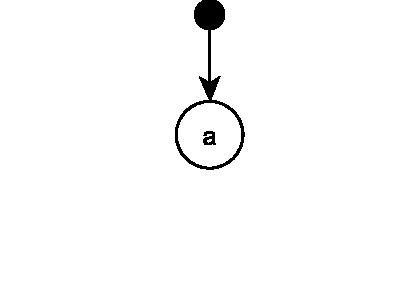
\includegraphics[width=\linewidth]{statechart_01}
    \caption{non-conflict}
    \label{fig:statechart_01}
  \end{subfigure}
  \hfill
  \begin{subfigure}[t]{0.32\linewidth}
    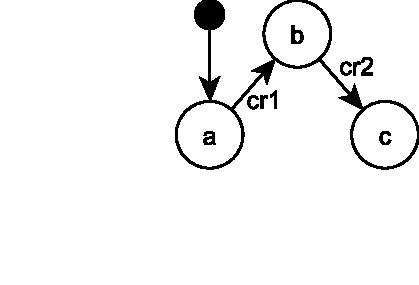
\includegraphics[width=\linewidth]{statechart_02}
    \caption{non-conflict}
    \label{fig:statechart_02}
  \end{subfigure}
  \hfill
  \begin{subfigure}[t]{0.32\linewidth}
    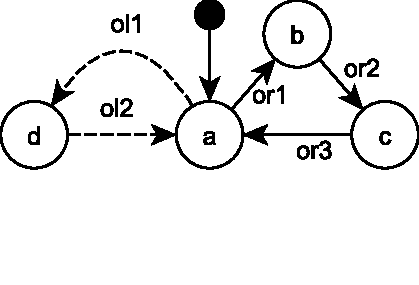
\includegraphics[width=\linewidth]{statechart_03}
    \caption{non-conflict}
    \label{fig:statechart_03}
  \end{subfigure}
  \\
  \begin{subfigure}[t]{0.32\linewidth}
    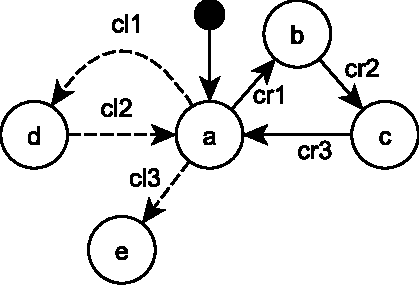
\includegraphics[width=\linewidth]{statechart_04}
    \caption{pseudo-conflict}
    \label{fig:statechart_04}
  \end{subfigure}
  \hfill
  \begin{subfigure}[t]{0.32\linewidth}
    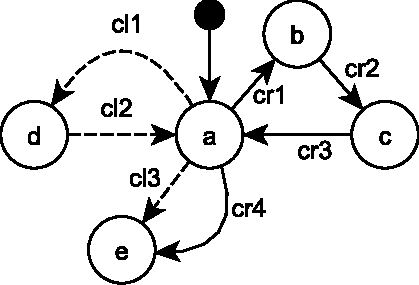
\includegraphics[width=\linewidth]{statechart_05}
    \caption{pseudo-conflict}
    \label{fig:statechart_05}
  \end{subfigure}
  \hfill
  \begin{subfigure}[t]{0.32\linewidth}
    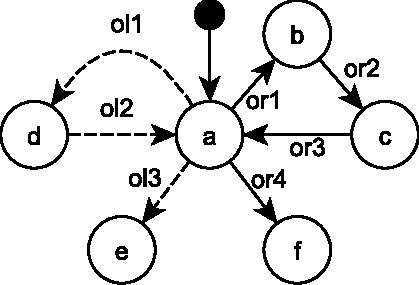
\includegraphics[width=\linewidth]{statechart_06}
    \caption{conflict}
    \label{fig:statechart_06}
  \end{subfigure}
  \caption{Conflicting and non-conflicting change events (dashed arrow = left change event, solid arrow = right change events, circle = state).}
  \label{fig:conflict_states}
\end{figure*}

Using (\ref{eq:ecbp_pseudoconflict}), condition in Figure \ref{fig:statechart_04} can be detected as a \textsf{PSEUDO} conflict. \textsf{PSEUDO} conflict means that a conflict can be automatically resolved. This means that we can automatically select one of the two conflicting change event sets as the applied change events without needing for human intervention. Since $C_{R}$ produces the eventual state that is equal to the original state, that is `a'; it does not have any effect -- the changes are not intended or cancelled. Thus, all its change events can be automatically negated. In other words, only change events in $C_{L}$ that are accepted to produce the eventual state, which is `e'. Also using (\ref{eq:ecbp_pseudoconflict}), condition is \ref{fig:statechart_05} can also be detected as another \textsf{PSEUDO} conflict. Both change event sets, $C_{L}$ and $C_{R}$, produce the same eventual state, `e', that is different from the original state, `a'. This can be automatically resolved since selecting one of the sets produces the same outcome. With (\ref{eq:ecbp_conflict}), the scenario in Figure \ref{fig:statechart_06} can be detected as a \textsf{REAL} conflict since change event sets, $C_{L}$ and $C_{R}$, produces two different eventual states. The conflict cannot be automatically resolved and requires user intervention to choose which one is the desired eventual state, `e' or `f', and then the appropriate change event set can be selected to produce the eventual state.


\subsection{Conflict Computation} 
\label{sec:conflict_computation} 
We perform procedure in Algorithm \ref{alg:conflict_detection} and employ (\ref{eq:ecbp_conflict}) and (\ref{eq:ecbp_pseudoconflict}) inside it to identify conflicts between two CBPs. Essentially, the algorithm works by iterating through all the elements, features, and values in the element three (Figure \ref{fig:right_element_tree_diagram}) and checking the equivalency of their original and eventual states as well the numbers of change events applied to them. The results are then used as inputs to decide whether a conflict has been detected or not.

\begin{table*}[ht]
  \centering
  \caption{Conflicting change events in Listings \ref{lst:cbp_left} and \ref{lst:cbp_right} identified using the proposed change-based conflict detection. The bold identifiers are the keys where the conflicts detected.}
  \label{table:conflicts_cbp}
  \begin{scriptsize}
  \begin{tabular}{|p{0.04\linewidth}|p{0.365\linewidth}|p{0.365\linewidth}|
      p{0.11\linewidth}|}
    \hline
    \textbf{ID} & 
    \textbf{Left Change Events (Bob)} & 
    \textbf{Right Change Events (Alice)} & 
    \textbf{Type}\\ 
    \hline
    CB1 & 
    set \textbf{troll.name} from "Troll" to "Ogre" & 
    set \textbf{troll.name} from "Troll" to "Orc" & 
    real \\
    \hline
    CB2 & move \textbf{target} in \textbf{character.parameters} from 1 to 2 & 
    move \textbf{target} in \textbf{character.parameters} from 1 to 0 & 
    real \\ 
    \hline
    CB3 & 
    \begin{minipage}[t]{\linewidth}
      \raggedright
      \begin{itemize}[leftmargin=0pt]
        \setlength
        \item[] unset cast.name from "cast" to null
        \item[] remove cast from giant.operations at 0
        \item[] delete cast type Operation
        \item[] unset giant.name from "Giant" to null
        \item[] delete \textbf{giant} type Class
      \end{itemize}
    \end{minipage}
    & 
    \begin{minipage}[t]{\linewidth}
      \raggedright
      \begin{itemize}[leftmargin=0pt]
        \setlength
        \item[] remove smash from knight.operations at 0
        \item[] add smash to \textbf{giant}.operations at 1
        \item[] remove cast from \textbf{giant}.operations at 0
        \item[] add cast to mage.operations at 0
      \end{itemize}
    \end{minipage}
    & 
    real, non-applicability\\
    \hline
    CB4 & 
    \begin{minipage}[t]{\linewidth}
      \raggedright
      \begin{itemize}[leftmargin=0pt]
        \setlength
        \item[] unset cast.name from "cast" to null
        \item[] remove cast from giant.operations at 0
        \item[] delete \textbf{cast} type Operation
        \item[] unset giant.name from "Giant" to null
        \item[] delete giant type Class
      \end{itemize}
    \end{minipage}
    & 
    \begin{minipage}[t]{\linewidth}
      \raggedright
      \begin{itemize}[leftmargin=0pt]
        \setlength
        \item[] remove \textbf{cast} from giant.operations at 0
        \item[] add \textbf{cast} to mage.operations at 0
      \end{itemize}
    \end{minipage}
    & 
    real, non-applicability\\
    \hline
    CB5 & 
    set \textbf{character.name} from "Character" to "Hero" & 
    set \textbf{character.name} from "Character" to "Hero" & 
    pseudo\\ 
    \hline
  \end{tabular}
\end{scriptsize}
\end{table*}
%------------------------------------------------------------------------------

The algorithm starts by creating an empty list \textsf{conflictList} to contain identified conflicts at line 2. The algorithm then iterates through all the elements, features, and values in the element tree. 

\subsubsection{Conflict with Deletion} 
\label{sec:delete_conflict} 
At lines 4 to 11 in Algorithm \ref{alg:conflict_detection}, the algorithm checks if there is a conflict related to a deletion of an element.
If an element is deleted on one or both sides, it means that all events related to the element on both sides should be in conflict. 
To get all the related events, the algorithm uses two functions,  \textsf{getAllRelatedLeftEvents($element$)} and \textsf{getAllRelatedRightEvents($element$)} (the element acts as a map key to access the change events), that return two sets of the related events, 
\textsf{leftEvents} and \textsf{rightEvents} respectively. The related events are events applied to the deleted element, including its sub-elements and features, 
and events that are parts of composite events. If both sets of events are not empty then a conflict is created containing both sets of events. 
If the element is deleted on both sides then we set the conflict as \textsf{PSEUDO}. The identified conflict is then added to \textsf{conflictList}.

\IncMargin{1.5em}
\begin{algorithm*}[]
  \begin{scriptsize}
  \SetKwInOut{Input}{input}
  \SetKwInOut{Output}{output}
  \Input{an instance of ElementTree $elementTree$}
  \Begin{
    $conflictList$ $\leftarrow$ ConflictList()\;
    \ForEach{$element$ \In $elementTree$}{
      \tcp{Handle conflicts with deletion ----------------------------}
      \If{isLeftDeleted($element$) \Or isRightDeleted($element$)}{
        $leftEvents$ $\leftarrow$ getAllRelatedLeftEvents($element$)\;
        $rightEvents$ $\leftarrow$ getAllRelatedRightEvents($element$)\;
        \If{size($leftEvents$) > 0 \AndA size($rightEvents$) > 0}{
          $conflict$ $\leftarrow$ createConflict($leftEvents$, $rightEvents$)\;
          \If{isLeftDeleted($element$) \AndA isRightDeleted($element$)}{
            setPseudo($conflict$)\;
          }
          addConflict($conflict$, $conflictList$)\;
          continue\;
        }
      }
      \tcp{Handle conflicts with cross-container move --------------------------}
      \If{(getOriginalContainer($element$) <> getLeftContainer($element$) \Or getOriginalContainingFeature($element$) <> getLeftContainingFeature($element$)) \Or
        (getOriginalContainer($element$) <> getRightContainer($element$) \Or getOriginalContainingFeature($element$) <> getRightContainingFeature($element$))}{
        $leftEvents$ $\leftarrow$ getAllRelatedLeftEvents($element$)\;
        $rightEvents$ $\leftarrow$ getAllRelatedRightEvents($element$)\;
        \If{size($leftEvents$) > 0 \AndA size($rightEvents$) > 0}{
          $conflict$ $\leftarrow$ createConflict($leftEvents$, $rightEvents$)\;
          \If{getLeftContainer($element$) = getRightContainer($element$) \AndA getLeftContainingFeature($element$) = getRightContainingFeature($element$}{
            setPseudo($conflict$)\;
          }
          addConflict($conflict$, $conflictList$)\;
        }
      }
      \ForEach{$feature$ \In getFeatures($element$)}{
        \tcp{Handle single-valued feature}
        handleSingleValuedFeature($element$, $feature$, $conflictList$)\;\label{line:conflict_single_value}
        \tcp{Handle multi-valued feature} 
        handleMultiValuedFeature($element$, $feature$, $conflictList$)\;\label{line:conflict_multi_value}
      }
    }
    \Return{$conflictList$}\;
  }
  \end{scriptsize}
  \caption{Algorithm for conflict detection using element tree.}
  \label{alg:conflict_detection}
\end{algorithm*}
\DecMargin{1.5em}

As an example, when the iteration reaches element \textsf{giant} in Figure \ref{fig:right_element_tree_diagram}, the algorithm identifies that the element has been deleted only on the left side.
Using the map in Table \ref{tab:keyeventsmap}, the algorithm then collects all the change events from both sides related to the element \textsf{giant} and its sub-elements. For key \textsf{giant}, it collects the change events at lines 39 to 42 for the left side and change events at lines 33 to 34 for the right side. For key \textsf{giant.name}, only left-side change event at line 40 is collected.
For key \textsf{giant.operations.cast}, it collects left-side change event at line 39 and right-side change event at line 34.
For key \textsf{giant.operations.smash}, only the right-side change event at line 33 is collected. 
For key \textsf{cast}, it collects change events at lines 38 to 40 for the left side and change events at lines 34 and 35 for the right side.
For key \textsf{giant.name}, it only left-side change event at line 38 is collected.
The collected change events are merged into one set of change events for each side. 
So, the left events are all events that comprise the composite event that deletes the element. 
The right events consist of events that move operation \textsf{smash} from class \textsf{knight} to class \textsf{giant} and events that
move operation \textsf{cast} from class \textsf{giant} to class \textsf{mage}. The algorithm then creates a conflict that consists of these events 
producing conflict \textsf{CB3} in Table \ref{table:conflicts_cbp}. 

When the iteration reaches element \textsf{cast} -- the operation of class \textsf{giant}, the same procedure is repeated. It collects left-side change events at lines 33, 38, 39, 40, 41, and 42, and right-side change events at lines 34, 35, and 38. The left-side change events related to element \textsf{giant} are also included since they are in one composite event that also affects element \textsf{cast}. These change events are collected into one conflict, \textsf{CB4}. 

It can be noticed that both conflicts \textsf{CB3} and \textsf{CB4} have shared change events. Thus these conflicts have a dependency to each other. It means that if a user chooses to delete \textsf{giant} -- choose the left side as the solution -- for conflict \textsf{CB3}, the left side change events also have to be selected as the solution for conflict \textsf{CB4} for consistency. To facilitate computing such dependencies, conflicts and change events are designed to have many-to-many relationships as depicted in Figure \ref{fig:approach_class_diagram}. Thus, if a change event is associated with two or more conflicts, it means that they depend on each other.

It is important to notice that at line 13 in Figure \ref{alg:conflict_detection} there is a command \textsf{continue} after the addition of a conflict caused by deletion. The command skips the iteration to the next element which avoids unnecessary conflict computation for the current element's  features and values. All change events related to the features and values have been collected by the functions \textsf{getAllRelatedLeftEvents($element$)} and \textsf{getAllRelatedRightEvents($element$)} at lines 5 and 6.  

\subsubsection{Conflict between cross-container Moves} 
\label{sec:move_conflict} 
Lines 15 to 25 in Algorithm \ref{alg:conflict_detection} are dedicated to identifying conflicts related to cross-container moves. 
First, the algorithm checks if an element has been moved from its original container to another container on one or both sides. 
If it does has been moved, 
it then checks the number of events related to the element by firstly obtaining change events related to the element on 
both sides using functions \textsf{getAllRelatedLeftEvents($element$)} and \textsf{getAllRelatedLeftEvents($element$)} yielding two sets of events, 
\textsf{leftEvents} and \textsf{rightEvents}. If the element has, at least, one event on each side,
a conflict is created containing \textsf{leftEvents} and \textsf{rightEvents}. 
If on both sides the element is moved to same container or the element is moved but finally returns to its original container on one of its sides then the conflict is set to \textsf{PSEUDO}.

  

\IncMargin{1.5em}
\begin{algorithm*}[]
  \begin{scriptsize}
    \SetKwInOut{Input}{input}
    \SetKwInOut{Output}{output}
    \Input{an element $element$}
    \Input{a feature $feature$}
    \Input{a list to contain conflicts $conflictList$}
    \Begin{
      \tcp{Handle single-valued feature --------------------------}
      \If{isSingleValued($feature$)}{
        $originalValue$ $\leftarrow$ getOriginalValue($feature$)\;
        $leftValue$ $\leftarrow$ getLeftValue($feature$)\;
        $rightValue$ $\leftarrow$ getRightValue($feature$)\;
        $leftEvents$ $\leftarrow$ getAllRelatedLeftEvents($element$, $feature$)\;
        $rightEvents$ $\leftarrow$ getAllRelatedRightEvents($element$, $feature$)\;
        \If{$originalValue$ <> $leftValue$ \Or $originalValue$ <> $rightValue$ \AndA size($leftEvents$) > 0 \AndA size($rightEvents$) > 0}{
          $conflict$ $\leftarrow$ createConflict($leftEvents$, $rightEvents$)\;
          \If{$leftValue$ = $rightValue$ \Or $leftValue$ = $originalValue$ \Or $rightValue$ = $originalValue$}{
            setPseudo($conflict$)\;
          }
          addConflict($conflict$, $conflictList$)\;
        }
      }
    }
  \end{scriptsize}
  \caption{Algorithm to handle single-valued feature in conflict detection using element tree -- handleSingleValuedFeature($element$, $feature$, $conflictList$) at line 27 in Algorithm \ref{alg:conflict_detection}.}
  \label{alg:conflict_single_valued_feature}
\end{algorithm*}
\DecMargin{1.5em}

\subsubsection{Single-valued Feature Conflict} 
\label{sec:single_valued_conflict}
Conflicts that involve single-valued features are handled by the procedure at line \ref{line:conflict_single_value} in Algorithm \ref{alg:conflict_detection}, which is elaborated in Algorithm \ref{alg:conflict_single_valued_feature}. The procedure starts by retrieving \textsf{leftValue}, \textsf{rightValue}, and \textsf{originalValue} of a single-valued feature. It then checks the inequality of \textsf{leftValue} and \textsf{rightValue} to \textsf{originalValue}. If one of \textsf{leftValue} and \textsf{rightValue} are not equal to \textsf{originalValue}, it then continues to check the number of change events related to the feature by firstly retrieving them using functions \textsf{getAllRelatedEvents($element$, $feature$)} and \textsf{getAllRelatedRightEvents($element$, $feature$)} (element and feature act as a map key to access the events) yielding two sets of related events, \textsf{leftEvents} and \textsf{rightEvents}. If \textsf{leftEvents} and \textsf{rightEvents} are not empty then a conflict that contains these events is instantiated. The procedure then checks the equality of \textsf{leftValue} and \textsf{rightValue} and sets the conflict to \textsf{PSEUDO} if \textsf{leftValue} and \textsf{rightValue} are equal or one of them is equal to \textsf{originalValue}. Finally, the conflict is put into \textsf{conflictList}. 

For example, when the iteration reaches feature \textsf{name} of class \textsf{troll}, the algorithm retrieves the left, right, and original values of the feature, yielding ``Ogre'', ``Orc'', and ``Troll'' respectively. Since ``Ogre'' and Orc'' are not equal to ``Troll'', the algorithm continues to retrieve two sets of events related to the feature. Only one event contained exists in each set. On the left side, the event sets the name of class \textsf{troll} from ``Troll'' to ``Ogre'', while on the right side, the the event sets it from ``Troll'' to ``Orc''. Both event sets are not empty thus a conflict containing them is created. Since ``Ogre'' is not equal to ``Orc'' the conflict is not set to \textsf{PSEUDO}. This conflict is the conflict \textsf{CB1} in Table \ref{table:conflicts_cbp}. This part of the algorithm also identifies conflict \textsf{CB5} except that this conflict is set to \textsf{PSEUDO} since both sides change class \textsf{character}'s \text{name} to a same value, ``Hero''. 



\IncMargin{1.5em}
\begin{algorithm*}[]
  \begin{scriptsize}
  \SetKwInOut{Input}{input}
  \SetKwInOut{Output}{output}
  \Input{an element $element$}
  \Input{a feature $feature$}
  \Input{a list to contain conflicts $conflictList$}
  \Begin{
    \tcp{Handle multi-valued feature --------------------------}
    \If{isMultiValued($feature$)}{
      \uIf{isOrdered($feature$)}{
        $values$ $\leftarrow$ getUnequalLeftAndRightValues($feature$)\;
        \ForEach{$value$ \In $values$}{
          $leftEvents$ $\leftarrow$ getAllRelatedLeftEvents($element$, $feature$, $value$)\;
          $rightEvents$ $\leftarrow$ getAllRelatedRightEvents($element$, $feature$, $value$)\;
          \If{size($leftEvents$) > 0 \AndA size($rightEvents$) > 0}{
            $conflict$ $\leftarrow$ createConflict($leftEvents$, $rightEvents$)\;
            \If{getLeftIndex($value$, $feature$) = getRightIndex($rightValue$, $feature$) \Or getLeftIndex($value$, $feature$) = getOriginalIndex($value$, $feature$) \Or getRightIndex($value$, $feature$) = getOriginalIndex($value$, $feature$)}{
              setPseudo($conflict$)\;
            }
            addConflict($conflict$, $conflictList$)\;
          }       
        }
      }\ElseIf{\Not isOrdered($feature$)}{
        $leftValues$ $\leftarrow$ getXORLeftAndOriginalValues($feature$)\;
        $rightValues$ $\leftarrow$ getXORRightAndOriginalValues($feature$)\;
        $values$ $\leftarrow$ $leftValues$ $\cup$ $rightValues$\;
        \ForEach{$value$ \In $values$}{
          $leftEvents$ $\leftarrow$ getAllRelatedLeftEvents($element$, $feature$, $value$)\;
          $rightEvents$ $\leftarrow$ getAllRelatedRightEvents($element$, $feature$, $value$)\;
          \If{size($leftEvents$) > 0 \AndA size($rightEvents$) > 0}{
            $conflict$ $\leftarrow$ createConflict($leftEvents$, $rightEvents$)\;
            \If{isLeftExisted($value$, $feature$) = isRightExisted($value$, $feature$) \Or isLeftExisted($value$, $feature$) = isOriginExisted($value$, $feature$) \Or isRightExisted($value$, $feature$) = isOriginExisted($value$, $feature$)}{
              setPseudo($conflict$)\;
            }
            addConflict($conflict$, $conflictList$)\;
          }       
        }
      }
    }
  }
\end{scriptsize}
  \caption{Algorithm to handle multi-valued feature in conflict detection using element tree -- handleMultiValuedFeature($element$, $feature$, $conflictList$) at line 28 in Algorithm \ref{alg:conflict_detection}.}
  \label{alg:conflict_multi_valued_feature}
\end{algorithm*}
\DecMargin{1.5em}

\subsubsection{Ordered Multi-valued Feature Conflict} 
\label{sec:ordered_conflict}
Conflicts that involve multi-valued features are handled by the procedure at line \ref{line:conflict_multi_value} in Algorithm \ref{alg:conflict_detection}, which is elaborated in Algorithm \ref{alg:conflict_multi_valued_feature}, where ordered multi-valued features are addressed at lines 3-15. The procedure relies on function \textsf{getUnequalLeftAndRightValues}. The function returns all values from left and right sides that are not equal to their original states in terms of (in)existence and indexes. For example, in Figure \ref{fig:right_element_tree_diagram}, parameter \textsf{target} in feature \textsf{parameters} is at index 2 on the left side but at index 1 in its original state. Thus, the value is included in the returned set. On the right side, this parameter is also at different index to its original index but it is already included in the returned set. 

The algorithm then iterates through the values of the set. For each value, it retrieves all events related to the value of this feature (element, feature, and value act as a map key to access the events) using functions \textsf{getAllRelated *Events($element$, $feature$, $value$)}, yielding two sets of events, \textsf{leftEvents} and \textsf{rightEvents}. If both sets of events are not empty then a conflict is created. If the value on both sides is at the same index then the conflict is \textsf{PSEUDO}. Lastly, the conflict is added to \textsf{conflictList}. The parameter \textsf{target} in feature \textsf{parameters} has been concurrently modified; it has one event on each side: parameter \textsf{target} is moved to the last index on the left side and to the first index on the right. Thus, a conflict in detected. This conflict is presented as conflict \textsf{CB2} in Table \ref{table:conflicts_cbp}.

%\begin{figure}[ht]
%    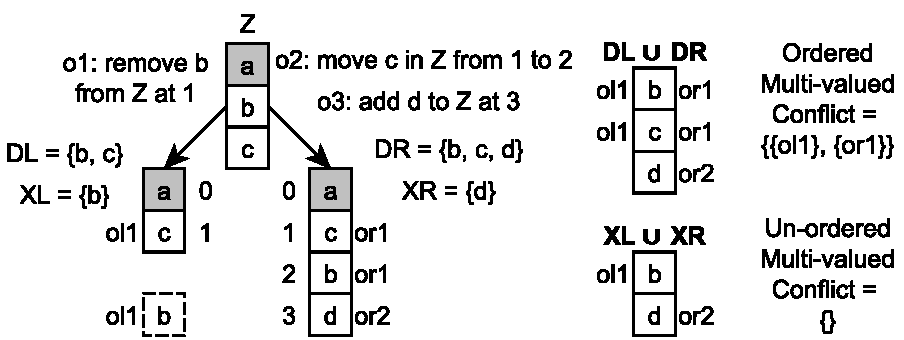
\includegraphics[width=\linewidth]{multi_valued_conflict_detection}
%    \caption{Detecting conflicts in Multi-valued features ($D$: values that are different at every index; $X$: XOR of values).}
%    \label{fig:multi_valued_conflict_detection}
%\end{figure}

\subsubsection{Unordered Multi-valued Feature Conflict} 
\label{sec:unordered_conflict}
Conflict detection for unordered, multi-valued features is handled at lines 16 to 29 in Algorithm \ref{alg:conflict_multi_valued_feature}. Instead of using function \textsf{getUnequalLeftAndRightValues}, it employs functions \textsf{getXOR*AndOriginalValues}. The functions also returns all values from left and right sides that are not equal to their original states but only in terms of (in)existence since indexing is not important in un-ordered features. The procedure to detect a conflict is similar to the procedure for ordered features. The difference is that, to determine if a conflict is \textsf{PSEUDO} or not, it checks the existence of values using functions \textsf{is*Existed}.

\section{Accuracy of Conflict Detection}
\label{sec:accuracy_of_conflict_detection}
Conflicts detected by EMF CBP, EMF Compare, and EMF Store can be different due to the different approaches employed by them. In this section, we explain in more detail the differences, firstly, between EMF CBP and EMF Compare, and secondly, between EMF CBP and EMF Store, on the conflicts they can/cannot detect. We use this classification of detected/undetected conflicts later in the evaluation to compare the accuracy of these tools.

\subsection{EMF CBP vs. EMF Compare}
\label{sec:emf_cbp_vs_emf_compare}
EMF Compare uses model differencing to derive changes -- not the real changes -- between two versions of a model. This can causes EMF Compare treats an element or feature as it has been modified even though in the real context no change has been applied to it, and further can lead EMF Compare to inaccurate conflict detection. On the other side, EMF CBP uses real recorded change events to determine conflicts thus its conflict detection is accurate. Following is the kinds of conflicts detected by EMF CBP but fail to be detected by EMF Compare. 
\begin{itemize}
  
  \item \emph{Real Move Conflict}. EMF CBP identifies accurately an element that has been moved, but EMF Compare picks another element. This case has been presented in the running example where EMF CBP detects that \textsf{target} has been moved on both sides (Conflict CB2, Table \ref{table:conflicts_cbp}), while EMF Compare identifies \textsf{target} and \textsf{gem} that have been moved on the left and right sides respectively (Listings \ref{lst:cbp_left_state} and \ref{lst:cbp_right_state}).
  
  \item \emph{One-sided Reset Conflict}. EMF CBP detects a \textsf{PSEUDO} conflict on an element or feature that simultaneously modified but then is set back to its original state on one of its sides (see Figure \ref{fig:statechart_04}). However, this condition is not detected as in conflict by EMF Compare since the states of the element or feature are the same both in the original and modified versions.   
  
  \item \emph{Single-valued Containment Conflict}. The change of state of a single-valued containment feature. EMF CBP detects two different changes are in conflict if they modify a single-valued containment feature concurrently. For example, element \textsf{e1} contained in \textsf{c1}.\textsf{value}, and element \textsf{e2} contained in \textsf{c2}.\textsf{value} are moved into \textsf{c3}.\textsf{value} concurrently, where \textsf{value} is a single-valued containment feature. Both changes are detected in conflict by EMF CBP but strangely not detected in conflict by EMF Compare.
\end{itemize}

Following is the only kind of conflicts detected by EMF Compare but fails to be detected by EMF CBP. 
\begin{itemize}
  \item \emph{Derived Move Conflict}. This conflict is the opposite of the Real Move conflict since EMF CBP only records real moves not the derived moves produced by EMF Compare. Thus EMF CBP cannot detect conflicts produced by derived moves.
\end{itemize}

\subsection{EMF CBP vs. EMF Store}
\label{sec:emf_cbp_vs_emf_store}
Even though both EMF CBP and EMF Store real records of changes to determine conflicts, EMF Store does not consider the eventual states of elements or features which leads to different conflicts detected by both. Following is the only kind of conflicts detected by EMF CBP but fails to be detected by EMF Store. 
\begin{itemize}
  \item \emph{First-time Move Conflict}. EMF Store can only identify a conflict between two different changes that modify an element concurrently in a multi-valued feature if both changes are the first changes applied to that multi-valued feature. If the there is an earlier change applied on another element in the same multi-valued feature, then the following two different changes on the same element do cause a conflict. For example, in the original version, a multi-valued feature \textsf{c1}.\textsf{children} contains elements \textsf{e1}, \textsf{e2}, and \textsf{e3}. If in the left version, \textsf{e2} is moved to the first position and, in the right version, \textsf{e2} is moved to the last position, then these concurrent changes are detected in conflict by EMF Store. However, if in the left version, the feature is modified with another change, let's say an addition of element \textsf{e4} at any position, both \textsf{move} changes are \textbf{not} detected in conflict by EMF Store. EMF CBP still detects both \textsf{move} changes in conflict.
\end{itemize}

Following is the only kind of conflicts detected by EMF Store but fails to be detected by EMF CBP. In other words, this conflicts should not be detected as conflicts by EMF Store.
\begin{itemize}
  \item \emph{Two-sided Reset Conflict}. These kind of conflicts is raised when two sets of changes modify an element or feature but reset its state to the original state on both sides. For example, in the left version, the value of attribute \textsf{e1}.\textsf{isEnabled} is set from \textsf{false} to \textsf{true}, but then it is set back again to \textsf{false}. In the right version, the same changes also applied on the same attribute. Thus, \textsf{e1}.\textsf{isEnabled} has eventual value \textsf{false} on both versions, the same value as in the original version. This kind of changes are treated in conflict by EMF Store but \textbf{not} a conflict in EMF CBP (see Figure \ref{fig:statechart_03}). The same rule also applies to an element that has been moved but then is moved back to its initial position.
\end{itemize}

Numbers of conflicts detected by EMF CBP and EMF Store can also be different due to grouping of dependent conflicts performed by EMF Store. For example, let's say that we have a model with initial state element \textsf{e1} contained in feature \textsf{c1}.\textsf{value} and two other empty features, \textsf{c2}.\textsf{value} and \textsf{c3}.\textsf{value}. On the left side, \textsf{e1} is moved twice; first, \textsf{e1} is moved to \textsf{c2}.\textsf{value} and then moved again to \textsf{c3}.\textsf{value} . The model is also modified on the right side; a new element \textsf{e2} is assigned to \textsf{c2}.\textsf{value}, and then another new element \textsf{e3} is assigned to \textsf{c3}.\textsf{value}. 

In this scenario, EMF CBP identifies two conflicts. The first conflict is a \textsf{PSEUDO} conflict (see Figure \ref{fig:statechart_04}) that is \textsf{c2}.\textsf{value} is concurrently modified on both sides but, on one side, the value is set back to its original state; on the right side, \text{e2} is assigned to \textsf{c2}.\textsf{value}, but, on the left side, \textsf{c2}.\textsf{value} is left back to empty due to the move of \textsf{e1} to \textsf{c3}.\textsf{value}. The second conflict is a \textsf{REAL} conflict, since \textsf{c3}.\textsf{value} is concurrently modified and have different values on both sides; on the left side, it contains \textsf{e1}, but, on the right side, it contains \textsf{e3}. EMF Store can also identifies these conflicts but they are merged into one conflict. Another example of conflict grouping can be found in Tables \ref{table:emfc_conflicts}, \ref{table:conflicts_emfs}, and \ref{table:conflicts_cbp}. Conflicts \textsf{EC3} and \textsf{EC4} in EMF Compare or conflicts \textsf{CB3} and \textsf{CB4} in EMF CBP are grouped into one conflict \textsf{ES4} in EMF Store since both are in the same composite event \textsf{l2}.

%\begin{figure*}
%    \begin{tabular}{l|c|r}
%        \begin{subfigure}[t]{0.31\linewidth}
%            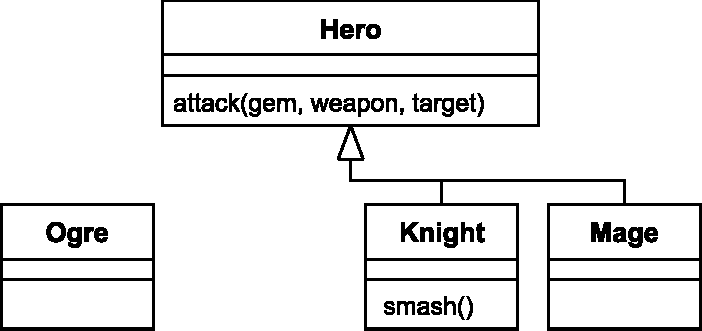
\includegraphics[width=\linewidth]{class_diagram_merged_ecbp}
%            \caption{EMF CBP}
%            \label{fig:class_diagram_merged_ecbp}
%        \end{subfigure}
%        &
%        \begin{subfigure}[t]{0.31\linewidth}
%            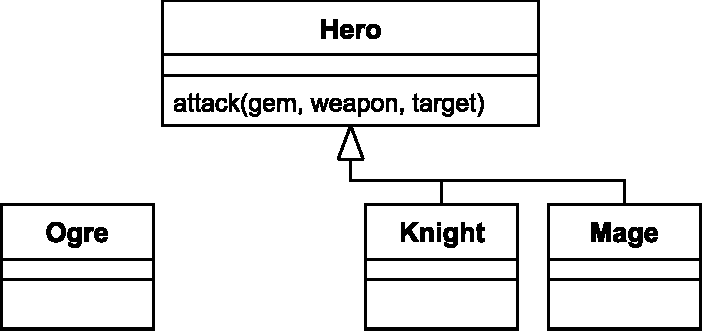
\includegraphics[width=\linewidth]{class_diagram_merged_emfc}
%            \caption{EMF Compare}
%            \label{fig:class_diagram_merged_emfc}
%        \end{subfigure}
%        &
%        \begin{subfigure}[t]{0.31\linewidth}
%            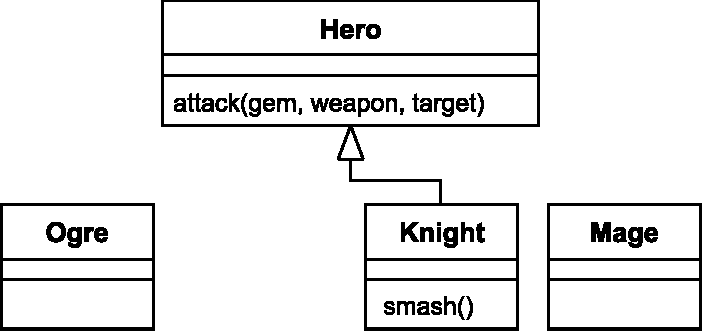
\includegraphics[width=\linewidth]{class_diagram_merged_emfs}
%            \caption{EMF Store}
%            \label{fig:class_diagram_merged_emfs}
%        \end{subfigure}
%    \end{tabular}
%    \caption{Merged models of models in Figure \ref{fig:class_diagram_rpg} after applying all-left-to-right merging.}
%    \label{fig:class_diagram_merged}
%\end{figure*}

%\section{Merging}
%\label{sec:merging}
%Conflict resolution and merging strategies are out of the scope of this paper. However, it is important to present the merged models of these three approaches in order inspect their correctness. Thus, we present the merged models of the models in Figure \ref{fig:class_diagram_rpg} using these three different approaches. The merge is all-left-to-right merge which means the left changes is prioritised above right changes. In other words, the right changes is applied first to the original model so that the left changes can override the right changes. If there is a conflict then the conflicting right changes are cancelled. In EMF Compare, this cancellation means only the left changes are executed, the right changes are \emph{not executed}, while, in EMF CBP and EMF Store, the right changes are \emph{reversed} so that the affected elements are brought back to their original states.    
%
%In the default implementation of EMF Compare, the all-left-to-right merge sets the right model as the target and the left model as the source. This means the left changes are not applied to the original model. Instead, they are applied to the right model. Using this strategy, if we resolve all the conflicts in Table \ref{table:conflicts_emfc} using the all-left-to-right merge, we get a merged model as in Figure \ref{fig:class_diagram_merged_emfc}. All the right events are not executed. Instead, in the right model, class \textsf{character}'s feature \text{name} is set to ``Hero'' and class \textsf{troll}'s feature \textsf{name} is set to ``Ogre''. Also, operation \textsf{cast} and class \textsf{giant} are removed from the right model. The removal of class \textsf{giant} also removes operation \textsf{smash} since the operation is contained by the class in the right model. 
%
%For EMF CBP and EMF Store, applying the all-left-to-right merging requires all the right events of the conflicts in Tables \ref{table:conflicts_emfs} and \ref{table:conflicts_cbp} to be reversed. This reversal brings back the states of the elements affected by the conflicting right events to their original states which makes the conflicting left events safe to be applied to the original model. All right events are applied first followed by the reversed conflicting right events and then by all left events (see Listings \ref{lst:cbp_merged_emfs} and \ref{lst:cbp_merged_ecbp}). In this order, the events are applied to the original model, not the right model as in the EMF Compare, to produce the merged model.
%
%\begin{lstlisting}[firstnumber=1,style=eol,caption={Merged change events of the models in Figure \ref{fig:class_diagram_rpg} and Listings \ref{lst:cbp_right} and \ref{lst:cbp_left} using EMF Store. The commented lines are added only to improve readability.},label=lst:cbp_merged_emfs]
%#--right events--
%move target in attack.parameters from 1 to 0
%remove smash from knight.operations at 0 composite l1
%add smash to giant.operations at 0 composite l1
%remove cast from giant.operations at 1 composite l2
%add cast to mage.operations at 0 composite l2
%create rightGen type Generalization
%set rightGen.general to character
%set troll.generalization to rightGen
%set character.name from "Character" to "Hero"
%remove rightGen from troll.generalization composite l3
%set mage.generalization to rightGen composite l3
%set troll.name from "Troll" to "Orc"
%#--reversed conflicting right events--
%set troll.name from "Orc" to "Troll"
%remove rightGen from mage.generalization composite l3r
%set troll.generalization to rightGen composite l3r
%set character.name from "Hero" to "Character"
%remove rightGen from troll.generalization
%set rightGen.general from character to null
%delete rightGen
%remove cast from mage.operations at 0 composite l2r
%add cast to giant.operations at 1 composite l2r
%remove smash from giant.operations at 0 composite l1r
%add smash to knight.operations at 0 composite l1r
%move target in attack.parameters from 0 to 1
%#--left events--
%create leftGen type Generalization
%set leftGen.general to character
%set troll.generalization to leftGen
%set character.name from "Character" to "Hero"
%remove leftGen from troll.generalization composite r1
%set knight.generalization to leftGen composite r1
%move target in attack.parameters from 1 to 2
%unset cast.name from "cast" to null composite r2
%remove cast from giant.operations at 0 composite r2
%delete cast composite r2
%unset giant.name from "Giant" to null composite r2
%delete giant comp r2
%set troll.name from "Troll" to "Ogre"
%\end{lstlisting}
%
%\vspace{-20pt}
%\begin{lstlisting}[firstnumber=1,style=eol,caption={Merged change events (operations) of the models in Figure \ref{fig:class_diagram_rpg} and Listings \ref{lst:cbp_right} and \ref{lst:cbp_left} using EMF CBP. The commented lines are added only to improve readability.},label=lst:cbp_merged_ecbp]
%#--right events--
%move target in attack.parameters from 1 to 0
%remove smash from knight.operations at 0 composite l1
%add smash to giant.operations at 0 composite l1
%remove cast from giant.operations at 1 composite l2
%add cast to mage.operations at 0 composite l2
%create rightGen type Generalization
%set rightGen.general to character
%set troll.generalization to rightGen
%set character.name from "Character" to "Hero"
%remove rightGen from troll.generalization composite l3
%set mage.generalization to rightGen composite l3
%set troll.name from "Troll" to "Orc"
%#--reversed conflicting right events--
%set troll.name from "Orc" to "Troll"
%remove cast from mage.operations at 0 composite l2r
%add cast to giant.operations at 1 composite l2r
%remove smash from giant.operations at 0 composite l1r
%add smash to knight.operations at 0 composite l1r
%move target in attack.parameters from 0 to 1
%#--left events--
%create leftGen type Generalization
%set leftGen.general to character
%set troll.generalization to leftGen
%set character.name from "Character" to "Hero"
%remove leftGen from troll.generalization composite r1
%set knight.generalization to leftGen composite r1
%move target in attack.parameters from 1 to 2
%unset cast.name from "cast" to null composite r2
%remove cast from giant.operations at 0 composite r2
%delete cast composite r2
%unset giant.name from "Giant" to null composite r2
%delete giant comp r2
%set troll.name from "Troll" to "Ogre"
%\end{lstlisting}
%
%The drawback of the EMF Compare approach is that it set the right model as the target for merging changes resulting the lost of operation \textsf{smash} in the merged model (Figure \ref{fig:class_diagram_merged_emfc}). In contrast, EMF CBP and EMF Store reverse the event that moves operation \textsf{smash} from class \textsf{knight} to class \textsf{giant} so that it moves back operation \textsf{smash} from class \textsf{giant} to class \textsf{knight}. The drawback of EMF Store is that it does not concern about the eventual states produced by the conflicting events. It only concern that a feature has been modified concurrently on both sides identified by the presence of, at least, an event on each side. For example, the eventual states of class \textsf{troll}'s feature \textsf{generalization} are \textsf{null} in the original, left, and right models. However, these are not considered by EMF Store. Instead, it only identifies that there are events on both sides associated to this feature. Thus, conflict \textsf{ES1} in \ref{table:conflicts_emfs} is generated. In consequence, all events related to the feature on the right side, and the events that are part of their composite events, are reversed resulting the exclusion of generalization \textsf{rightGen} from the merged model. This drawback has been addressed by the EMF CBP by checking the equality of the original, left, and right states of the feature. Since they are all equal then there is no conflict between the events. Thus, EMF CBP produces a merged model as in Figure \ref{fig:class_diagram_merged_ecbp}.


\section{Evaluation Method}
\label{sec:evaluation_method}
This section presents the method that was employed to evaluate the change-based conflict detection approach proposed in this study and discuss the results. In order to assess the performance benefits of the proposed conflict detection, this study has evaluated it against a mature and widely-used state-based model comparison tool, EMF Compare \cite{emfcompare2018developer,eclipse2017compare}, and another implementation of change-based model persistence, EMF Store \cite{koegel2010emfstore}.

Since there are no manually developed, large models persisted in the proposed change-based format yet, the dataset for this experiments was constructed from a large model reverse-engineered from the Eclipse Epsilon project \cite{eclipse2018epsilongit,eclipse2017epsilon}. This model conforms to the Java metamodel \cite{eclipse2018modiscojava} and consists of more than 500 thousand elements with a size of 71.1 MBs when persisted in XMI. We aimed for larger sizes of models, but, due to slow execution of replaying change events event in EMF Store, we stayed with the current sizes as they are large enough to identify clearly the performance gaps between the approaches.

The original model was cloned to produce two new (left and right) models and perform operations (\textsf{add}, \textsf{remove}, \textsf{move}, \textsf{set} with random elements, features, indexes, and values) on both models to create differences. In the evaluation, 0.44 million artificial changes were applied to each model, generating almost 0.5 million events (one operation can generate more than one event, e.g. a \textsf{move} between features generates \textsf{remove} and \textsf{add} events). Events generated by the changes were persisted in the proposed change-based format (to be used later in change-based model comparison). After every 20,000 changes, a measurement point is made. The eventual state of the models were persisted in state-based format (to be used later in state-based model comparison), and changes persisted in EMF CBP were  also replayed on EMF Store to produce equivalent changes. After that, conflict detection using EMF Compare, EMF Store, and EMF CBP were performed and their execution time and memory footprint were measured. In one experiment, 22 measurement points were analysed to capture their trends. 

This evaluation conducted five experiments to evaluate the model conflict detection of the proposed approach. In the first experiment, the ratio of occurrence between \textsf{add}, \textsf{remove}, \textsf{move}, and \textsf{set} changes is set to 1:1:20:40 reflecting the assumption that, in a mature model, \textsf{move} and \textsf{set} events occur more frequent than addition and deletion. To reduce the effect of the change on the number of total elements to our measurement, the number of total elements should be kept constant. For example, it is difficult to tell an increase of time in comparison is caused by an increase in the number of elements or by the number of change events. One way to do this was to exclude \textsf{add} and \textsf{remove} operations. However, excluding both operations made measurement less representative. Thus, both operations were still included but their probabilities were made equal so that the number of total elements remain largely unchanged. In the rest of the experiments,
homogeneous type change events -- isolated from other types -- were performed per experiment (e.g. add-only, move-only change events). In the end, 5 results of the experiments were obtained: mixed, add-only, remove-only, move-only, and set-only measurement results. They are useful to assess whether operations of different types have a different impact on model comparison. For the delete-only experiment on EMF Store, due to slow execution of replaying \textsf{delete} event in EMF Store, the size of the models was reduced from 0.54 million to only 39.5 thousand elements each, and the number of changes from 0.44 millions to 33 thousands in 22 measurement points -- 1.5 thousand changes for each measurement point.

For conflict detection in EMF CBP, the conflict detection time comprises loading change events, constructing an element tree, and computing conflicts. The memory footprint is the space used to hold the change events, element tree, and conflicts in memory. For EMF Compare, the comparison time comprises matching elements and identifying differences, and the memory footprint is the space required to hold the matches and differences in memory. For EMF Store, the conflict detection time comprises loading and mapping change events and computing conflicts. The memory footprint is the space used to hold the change events and mapping and conflicts in memory.

To evaluate the accuracy of conflict detection of EMF CBP, EMF Compare, and EMF Store, we took the change events and states of models produced at the last measurement point of the mixed-operation experiment, and used them to analyse the conflicts detected by the three tools based on the classification in Section \ref{sec:accuracy_of_conflict_detection}.

All measurements were performed on the same machine and software with the following specification: Intel(R) Xeon(R) CPU E5-2680 v4 @ 2.40GHz (56 processors), 528 GBs main memory, Ubuntu 16.04.6 LTS operating system, OpenJDK Runtime Environment (build 1.8.0\_222-8u222-b10-1ubuntu2~16.04.york0-b10) with JVM \textsf{InitialHeapSize} 2 GBs and \textsf{MaxHeapSize} 32 GBs, EMF Store 1.9.0, EMF Compare 3.3.2, MoDisco 1.0.1, and EMF 2.12.0.

\section{Evaluation Results and Discussion}
\label{sec:evaluation_discussion}
This section reports and discuss the results obtained from the evaluation in terms of execution time and memory footprint of EMF CBP, EMF Compare, and EMF Store in detecting conflicts. 

\subsection{Mixed Operations}
\label{sec:mixed-operation_conflict}

In the mixed operation measurement, we modify two identical models differently by applying random operations. As the number of change events generated by the modification grows, the numbers of affected elements and differences also increase in a logarithmic manner. The patterns can be seen in Figure \ref{fig:conflict-size-events}. The growth is logarithmic since the probability that the random operations modify the same elements also increases. Thus, some change events might not contribute to the addition of new affected elements and differences. In other words, more events are required to increase the number of affected elements or differences. In Figure \ref{fig:conflict-size-events}, the total elements remains largely unchanged due to the equal probabilities of addition and deletion as has been set in Section \ref{sec:evaluation_method}. The figure gives us an insight about the characteristics of the modification caused by the random operations in the mixed operation measurement; it supports explaining the implication of the changes on execution time and memory footprints of model comparison.

The growing number of change events in the conflict detection evaluation is followed by the logarithmic increase of affected elements (Figure \ref{fig:conflict-size-events}). The total number of both elements can also be kept relatively constant due to 1:1 ratio of \textsf{add} and \textsf{delete} operations' occurrence. These change events produce different numbers of conflicts for EMF CBP, EMF Compare, and EMF Store as can be seen in Figure \ref{fig:conflict-count-events}. The differences are due to their distinct conflict detection approaches. EMF Compare detects fewer conflicts than EMF CBP and EMF Store since its change events are derived, not the real changes. EMF Store detects fewer conflicts than EMF CBP since its conflicts that depends to each other are grouped into one conflict.

Figure \ref{fig:conflict-time-events} exhibits EMF CBP outperforms EMF Compare and EMF Store in terms of execution time in detecting conflicts, even when the number of change events approaching a million. EMF Store is the slowest. It takes more than 35 seconds even though the number of change events has just reached 0.1 millions. Figure \ref{fig:conflict-memory-events} also shows EMF CBP outperforms EMF Compare and EMF Store in terms of memory footprint in conflict detection. At the last measurement point, a million change events, EMF CBP only consumes 6 GBs which is much less than EMF Compare and EMF Store. EMF Compare occupies around 16 GBs while EMF Store already consumes the same amount of memory footprint only for 0.5 million change events.

\begin{figure*}[]
  \centering
  \begin{minipage}[b]{0.490\textwidth}
    \includegraphics[width=\linewidth]{ecbp-conflict-time-events}
    \caption{A breakdown view of EMF CBP on the time required for conflict detection.}
    \label{fig:ecbp-conflict-time-events}    
  \end{minipage}
  \hfill
  \begin{minipage}[b]{0.490\textwidth}
    \includegraphics[width=\linewidth]{ecbp-conflict-memory-events}
    \caption{A breakdown view of EMF CBP on the memory footprint for conflict detection.}
    \label{fig:ecbp-conflict-memory-events}    
  \end{minipage}  
\end{figure*}

\begin{figure*}[]
  \centering
  \begin{minipage}[b]{0.490\textwidth}
    \includegraphics[width=\linewidth]{emfc-conflict-time-events}
    \caption{A breakdown view of EMF Compare on the time required for conflict detection.}
    \label{fig:emfc-conflict-time-events}
  \end{minipage}
  \hfill
  \begin{minipage}[b]{0.490\textwidth}
    \includegraphics[width=\linewidth]{emfc-conflict-memory-events}
    \caption{A breakdown view of EMF Compare on the memory footprint for conflict detection.}
    \label{fig:emfc-conflict-memory-events}
  \end{minipage}
\end{figure*}

\begin{figure*}[]
  \begin{minipage}[b]{0.490\textwidth}
    \includegraphics[width=\linewidth]{emfs-conflict-time-events}
    \caption{A breakdown view of EMF Store on the time required for conflict detection.}
    \label{fig:emfs-conflict-time-events}
  \end{minipage}
  \hfill
  \begin{minipage}[b]{0.490\textwidth}
    \includegraphics[width=\linewidth]{emfs-conflict-memory-events}
    \caption{A breakdown view of EMF Store on the memory footprint for conflict detection.}
    \label{fig:emfs-conflict-memory-events}
  \end{minipage}
\end{figure*}

Figures \ref{fig:ecbp-conflict-time-events}, \ref{fig:emfc-conflict-time-events}, and \ref{fig:emfs-conflict-time-events} show the detailed view of EMF CBP, EMF Compare, and EMF Store on the time required to complete conflict detection. As can be seen in Figure \ref{fig:ecbp-conflict-time-events}, the time for EMF CBP to load change events, construct the element tree, and detect conflicts grows linearly. In detecting conflicts, the EMF CBP does not require to perform differencing since changes are already available in the form of change events. Thus, differencing is not included in the diagram. 

In EMF Compare (Figure \ref{fig:emfc-conflict-time-events}), we can notice that the time taken for matching is less than 5 seconds, and the time used for identifying differences is around 15 seconds in average. The differencing takes a great portion of the time since it needs to derive differences twice; differences between left and original models and right and original models. The time for for matching and differencing tends to be constant since the sizes of the models are set to be as constant as possible (Figure \ref{fig:conflict-size-events}). In contrast, the time for detecting conflicts tends to incline due to the increasing number of conflicting changes as the number of change events increases. In detecting conflicts, EMF Store allocates most of the consumed time for identifying conflicts, and the time increases exponentially. The rest of the time is used for loading changes and mapping them to their affected elements and features (Figure \ref{fig:emfs-conflict-time-events}). 

In terms of memory footprint, EMF CBP allocates most of the memory space for element tree construction and the rest is for the loading change events and identifying conflicts (Figure \ref{fig:ecbp-conflict-memory-events}). The reason for this is due to our technical implementation in constructing \textsf{elementTree}. A Feature can have many instances even though they refer to the same feature. This causes the memory to increase. One solution is to construct a partial metamodel so that a feature can only have one instance and the instance is used as a key to access the feature's values in each element, similar to the implementation of feature in EMF Framework. In EMF Compare (Figure \ref{fig:emfc-conflict-memory-events})), the amount of memory used for matching and differencing only increases slightly due to the sizes of the models that are set to be as constant as possible (Figure \ref{fig:conflict-size-events}). In contrast, the memory used for detecting conflict increases as the number of detected conflicts rises (Figure \ref{fig:conflict-count-events}). For EMF Store, the amount of memory used for loading changes and mapping increases slightly while the amount of memory for identifying conflicts grows exponentially (Figure \ref{fig:emfs-conflict-memory-events}).



From the last measure point of the mixed-operation experiment, there are around 91 thousand conflicts detected by EMF Compare, and around 3 thousands (3.3\%) of them cannot be detected by EMF CBP. This is due to the derived move changes produced by EMF Compare, which are different from the real changes recorded by EMF CBP. In contrast, EMF CBP detects around 107 thousand conflicts, and there are around 19 thousand (18\%) conflicts that cannot be detected by EMF Compare; the number consists of 6.6 thousand (6.6\%) real move conflicts, 8.2  thousand (7.6\%) one-sided reset conflicts, and 4.1 thousand (3.8\%) single-valued containment conflicts (see Section \ref{sec:emf_cbp_vs_emf_compare} to find the definitions of these kinds of conflicts). Thus, there are 88 thousand (91 - 3 = 107 - 19 thousands) conflicts can be detected by both.

From 107 thousand conflicts detected by EMF CBP, there are 3.7 million (3.5\%) conflicts that cannot be detected by EMF Store which is caused by the first-time move conflict (see Section \ref{sec:emf_cbp_vs_emf_store}). By contrast, EMF CBP cannot detect 1.8 thousands (1.8\%) of the 96.4 thousand conflicts detected by EMF Store due to the two-sided reset conflicts (see Section \ref{sec:emf_cbp_vs_emf_store}). 

\begin{figure*}[ht]
  \centering
  \begin{subfigure}[t]{0.490\linewidth}
    \includegraphics[width=\linewidth]{add-conflict-time-events}
    \caption{add-only}
    \label{fig:add-conflict-time-events}
  \end{subfigure}
  \hfill
  \begin{subfigure}[t]{0.490\linewidth}
    \includegraphics[width=\linewidth]{delete-conflict-time-events}
    \caption{delete-only}
    \label{fig:delete-conflict-time-events}
  \end{subfigure}
  \\
  \begin{subfigure}[t]{0.490\linewidth}
    \includegraphics[width=\linewidth]{move-conflict-time-events}
    \caption{move-only}
    \label{fig:move-conflict-time-events}
  \end{subfigure}
  \hfill
  \begin{subfigure}[t]{0.490\linewidth}
    \includegraphics[width=\linewidth]{change-conflict-time-events}
    \caption{change-only}
    \label{fig:change-conflict-time-events}
  \end{subfigure}
  \caption{Conflict detection time for homogeneous operations.}
  \label{fig:homgeneous_operation_time_events}
\end{figure*}

\subsection{Homogenous Operations}
\label{sec:homogenous-operation_conflict}

\subsubsection{Detection Time} 
\label{sec:detection_time}
Figure \ref{fig:homgeneous_operation_time_events} depicts the results of conflict detection time between EMF CBP, EMF Compare, and EMF Store in homogenous operations. The results show that, in all types of homogenous operations, EMF CBP is faster at detecting conflicts compared to EMF Compare and EMF Store. The latter has the worst performance in most cases except in the delete-only experiment. In this case, EMF Compare is the slowest. EMF Compare also requires to calculate dependencies between conflicts. So, when the number of deletions is excessive, EMF Compare performs less efficiently than EMF Store (Figure \ref{fig:delete-conflict-time-events}). In the evaluation, this happens when the number of change events exceeds 240 thousands.

\begin{figure*}[ht]
  \centering
  \begin{subfigure}[t]{0.490\linewidth}
    \includegraphics[width=\linewidth]{add-conflict-memory-events}
    \caption{add-only}
    \label{fig:add-conflict-memory-events}
  \end{subfigure}
  \hfill
  \begin{subfigure}[t]{0.490\linewidth}
    \includegraphics[width=\linewidth]{delete-conflict-memory-events}
    \caption{delete-only}
    \label{fig:delete-conflict-memory-events}
  \end{subfigure}
  \\
  \begin{subfigure}[t]{0.490\linewidth}
    \includegraphics[width=\linewidth]{move-conflict-memory-events}
    \caption{move-only}
    \label{fig:move-conflict-memory-events}
  \end{subfigure}
  \hfill
  \begin{subfigure}[t]{0.490\linewidth}
    \includegraphics[width=\linewidth]{change-conflict-memory-events}
    \caption{change-only}
    \label{fig:change-conflict-memory-events}
  \end{subfigure}
  \caption{Conflict detection memory for homogeneous operations.}
  \label{fig:homgeneous_operation_memory_events}
\end{figure*}

\subsubsection{Memory Footprint}
\label{sec:memory_footprint}
Figure \ref{fig:homgeneous_operation_memory_events} illustrates the memory footprint resulting from conflict detection in EMF CBP, EMF Compare, and EMF Store with homogeneous operations. The Figure displays that EMF CBP outperforms EMF Compare and EMF Store in terms of memory footprint. EMF CBP only performs worse than EMF Compare in the delete-only experiment when the number of change events is more than 80 thousands -- model size is 39.5 thousand elements each (Figure \ref{fig:delete-conflict-memory-events}). In terms of memory footprint, EMF Store performs worse than EMF CBP and EMF Compare. It only performs better than EMF Compare when the number of change events is relatively small -- less than 25 thousand change events. 



In Figure \ref{fig:move-conflict-memory-events}, EMF CBP's memory footprint tends to increase faster than EMF Compare's memory footprint. This is possible since the change events of EMF Compare are actually minimal differences that are derived from model differencing which in terms of number is less than real change events recorded in EMF CBP. More random change events means higher possibility to produce more conflicts.

\subsubsection{Conflict Count}
\label{sec:conflict_count}
Figure \ref{fig:homgeneous_operation_count_events} displays the number of conflicts, both \textsf{REAL} and \textsf{PSEUDO}, detected by EMF CBP, EMF Compare, and EMF Store in the context of homogenous operations. In the add-only experiment as displayed in Figure \ref{fig:add-conflict-count-events}, all of them detect the same number of conflicts.

\begin{figure*}[ht]
  \centering
  \begin{subfigure}[t]{0.490\linewidth}
    \includegraphics[width=\linewidth]{add-conflict-count-events}
    \caption{add-only}
    \label{fig:add-conflict-count-events}
  \end{subfigure}
  \hfill
  \begin{subfigure}[t]{0.490\linewidth}
    \includegraphics[width=\linewidth]{delete-conflict-count-events}
    \caption{delete-only}
    \label{fig:delete-conflict-count-events}
  \end{subfigure}
  \\
  \begin{subfigure}[t]{0.490\linewidth}
    \includegraphics[width=\linewidth]{move-conflict-count-events}
    \caption{move-only}
    \label{fig:move-conflict-count-events}
  \end{subfigure}
  \hfill
  \begin{subfigure}[t]{0.490\linewidth}
    \includegraphics[width=\linewidth]{change-conflict-count-events}
    \caption{change-only}
    \label{fig:change-conflict-count-events}
  \end{subfigure}
  \caption{Conflict detection count for homogeneous operations.}
  \label{fig:homgeneous_operation_count_events}
\end{figure*}

Figure \ref{fig:change-conflict-count-events} shows the results of the change-only experiment. We can notice that the number of conflicts detected by EMF Compare is lower than EMF CBP. This is mainly due to EMF Compare detects no change on an element or feature that has been modified but finally changed back to its original state. While in EMF CBP, this is counted as a change with potential to raise a {PSEUDO} conflict as defined and showed in (\ref{eq:ecbp_pseudoconflict}), Section \ref{sec:emf_cbp_vs_emf_compare}, and Figure \ref{fig:statechart_04}. At the last measurement point in Figure \ref{fig:change-conflict-count-events}, there are 17 thousands (13.1\% of 130 thousand EMF CBP conflicts) of this kind of conflict undetected by EMF Compare. EMF Compare itself only detects 113 thousand conflicts. 

It can also be noticed that the number of conflicts detected by EMF CBP is slightly less than EMF Store detects. This happens because, as previously discussed, EMF Store does not consider states in detecting conflicts thus two different change events that are applied to a same element or feature, even though they yield eventual states that are equal to their original state, are considered in conflict. In Figure \ref{fig:change-conflict-count-events}, at the last measurement point, in total, EMF Store detects 133 thousand conflicts but 3.1 thousands (2.3\%) of them cannot be detected by EMF CBP due to this two-sided reset conflict (see Section \ref{sec:emf_cbp_vs_emf_store}). 

In the delete-only experiment in Figure \ref{fig:delete-conflict-count-events}, EMF CBP and EMF Compare detect more conflicts than EMF Store since they do not put a conflict that depends on another conflict into one group as performed by EMF Store as has been discussed in Section \ref{sec:emf_cbp_vs_emf_store}. As the number of change events grows, the number of conflicts that share the same change events also increases. Thus, these conflicts are grouped into one conflict causing the number of conflicts decreasing (see Section \ref{sec:emf_cbp_vs_emf_store}). In addition, EMF CBP detects fewer conflicts than EMF Compare since it skips calculating conflicts for features and values of an element that have been deleted. Change events that affect the features and values have been included when calculating conflicts caused by the deletion of the element as been explained in the last paragraph of Section \ref{sec:delete_conflict}. In contrast, EMF Compare treats the conflicts at the features and values of a deleted element as separate conflicts. 

Figure \ref{fig:move-conflict-count-events} shows the results of the move-only experiment. EMF CBP detects more conflicts than EMF Compare since it has more change events than EMF Compare due to the use of real records of changes. In EMF Compare, its change events are derived and effective which means minimum number of change events are produced. Less number of change events means less probable to produce conflicts. EMF Store detects fewer conflicts than EMF CBP and EMF Compare due to grouping of conflicts that depend to each other as has discussed in Section \ref{sec:emf_cbp_vs_emf_store}.

Using the data of conflicts from the last measurement point in Figure \ref{fig:move-conflict-count-events}, we identify that, from 91.6 thousand conflicts detected by EMF Compare, 4.7 thousands (5.1\%) of them are derived move conflicts which cannot be detected by EMF CBP. By contrast, from 114.8 thousand conflicts detected by EMF CBP, there are 27.9 million (24.3\%) conflicts cannot be detected by EMF Compare, consisting of 20.3 thousand (17.7\%) real move conflicts and 7.6 thousand (6.6\%) single-valued containment conflicts (see Section \ref{sec:emf_cbp_vs_emf_compare}). We also identify that, from 115 thousand conflicts detected by EMF CBP, 17 thousands (14.8\%) of them are undetected by EMF Store due to the first-time move conflict explained in Section \ref{sec:emf_cbp_vs_emf_store}. On the other hand, from all 29.5 thousand conflicts detected by EMF Store, only 2.5 thousands (8.5\%) of them cannot be detected by EMF CBP due to the two-sided reset conflict presented in Section \ref{sec:emf_cbp_vs_emf_store}.

\subsection{Conclusions}
\label{sec:conclusions_7}
In this chapter, we have presented an approach to speed up model conflict detection by exploiting the nature of change-based persistence which allows us to find conflicts between versions of a model only by comparing the last set of changes between the two versions. Based on the findings in the conflict detection evaluation, this study found that the proposed change-based model conflict detection approach outperforms the conflict detection approaches in EMF Compare and EMF Store. Nevertheless, models that have been excessively modified or experience significant reduction on model size could impair the performance of the conflict detection as a great number of change records have to be read and loaded into memory.

This chapter has addressed the third research question of this study, \textbf{Following change-based model differencing, how can conflicts be detected between versions of a model, and  how does change-based conflict detection perform, in terms of speed and memory, compared to state-based model conflict detection?} (RQ3). Similar to change-based model differencing, this work also has proposed an approach to model conflict detection by exploiting the nature of change-based persistence which allows us to detect conflict between two versions of a model only by comparing the eventual states of elements and features of the two versions, including their shared original version, that are affected by change events.

The phases in the change-based conflict detection are similar to the phases (event loading, element tree construction, and diff computation) in the change-based model differencing except that the diff computation is replaced with conflict computation. It also consists of a set of rules that compare the eventual states of the elements and features in the element tree as well as the number of change events that affects them in both versions. As an example, a feature that is modified only in one version cannot have conflicts. A conflict only occurs if the feature is modified on both versions. Also since the element tree also records every change event to the elements of features that it affect, we can trace change events that cause a conflict.

